\documentclass[10pt]{article}
\usepackage[vietnamese]{babel}
\usepackage[utf8]{inputenc}
\usepackage[T5]{fontenc}
\usepackage{graphicx}
\usepackage[export]{adjustbox}
\graphicspath{ {./images/} }
\usepackage{amsmath}
\usepackage{amsfonts}
\usepackage{amssymb}
\usepackage[version=4]{mhchem}
\usepackage{extpfeil}
\usepackage{stmaryrd}
\usepackage{bbold}

%New command to display footnote whose markers will always be hidden
\let\svthefootnote\thefootnote
\newcommand\blfootnotetext[1]{%
  \let\thefootnote\relax\footnote{#1}%
  \addtocounter{footnote}{-1}%
  \let\thefootnote\svthefootnote%
}

%Overriding the \footnotetext command to hide the marker if its value is `0`
\let\svfootnotetext\footnotetext
\renewcommand\footnotetext[2][?]{%
  \if\relax#1\relax%
    \ifnum\value{footnote}=0\blfootnotetext{#2}\else\svfootnotetext{#2}\fi%
  \else%
    \if?#1\ifnum\value{footnote}=0\blfootnotetext{#2}\else\svfootnotetext{#2}\fi%
    \else\svfootnotetext[#1]{#2}\fi%
  \fi
}

\begin{document}
\begin{center}
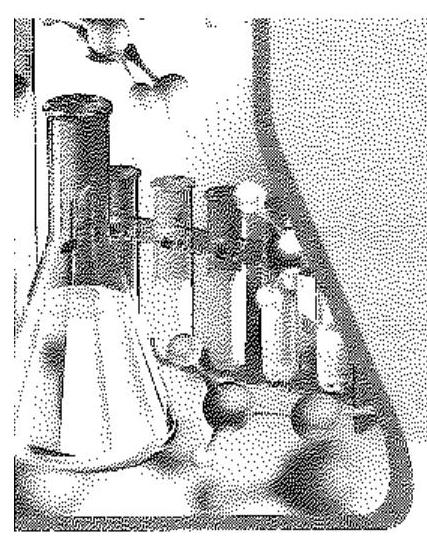
\includegraphics[max width=\textwidth]{2025_10_23_3f52bbaab6caa9e2ff75g-01}
\end{center}

\section*{ĐÁP ÁN VÀ HƯỚNG DẪN TRẢ LỜI}
\section*{BÀl 1}
1.1. a) (1)-OH; (2)-COOH; (3)-OR.\\
b) (4) tế bào sống: (5) nước; (6) không phân cực.\\
c) (7) triester; (8) glycerol; (9) triglyceride.\\
d) (10) monocarboxylic acid; (11) không phân nhánh; (12) chẵn.\\
1.2. A.\\
1.3. A.\\
1.4. D.\\
1.5. B.\\
1.6. C.\\
1.7. B.\\
1.8. A.\\
1.9. B.\\
1.10. B\\
1.11.C.\\
1.12. (a), (c).\\
1.13. C.\\
1.14. (a), (c), (d), (e), (h), (i).\\
1.15. B. $\mathrm{n}_{\mathrm{x}}=\mathrm{n}_{\mathrm{NaOH}}=0,03 \mathrm{~mol}$. Khối lượng mol của ester X là: $\frac{2,64}{0,03}=88\left(\mathrm{~g} \mathrm{~mol}^{-1}\right)$.

Gọi công thức của ester X là $\mathrm{C}_{\mathrm{n}} \mathrm{H}_{2 \mathrm{n}} \mathrm{O}_{2}$. Ta có: $14 \mathrm{n}+32=88 \Rightarrow \mathrm{n}=4$.\\
Công thức phân tử của X là $\mathrm{C}_{4} \mathrm{H}_{8} \mathrm{O}_{2}$.\\
1.16. Gọi công thức của X là $\mathrm{C}_{\mathrm{x}} \mathrm{H}_{\mathrm{y}} \mathrm{O}_{2}$. Ta có: $\mathrm{x}=\frac{60.100}{100.12}=5$ và $\mathrm{y}=\frac{8.100}{100.1}=8$.

Công thức phân tử của X là $\mathrm{C}_{5} \mathrm{H}_{8} \mathrm{O}_{2} . \mathrm{X}$ là ester tạo bởi carboxylic acid mạch phân nhánh nên X là $\mathrm{CH}_{2}=\mathrm{C}\left(\mathrm{CH}_{3}\right) \mathrm{COOCH}_{3}$.

Tên của $\mathbb{X}$ là methyl methacrylate.\\
1.17. Số mol acetic acid là: $\frac{4,00.1,05}{60}=0,07(\mathrm{~mol})$.

Số mol isoamyl alcohol 1à: $\frac{8,00.0,81}{88}=0,074(\mathrm{~mol})$. Như vậy, isoamyl alcohol du.

Số mol isoamyl acetate sinh ra theo lí thuyết $=$ số mol acetic acid $=0,07 \mathrm{~mol}$ Số mol isoamyl acetate thực tế thu được là: $\frac{6,00.0,88}{130}=0,041(\mathrm{~mol})$ Hiệu suất phản úng ester hoá là: $\frac{0,041}{0,07} \cdot 100 \%=58,571 \%$.\\
1.18. a) Gọi công thức phân tử của X là $\mathrm{C}_{\mathrm{x}} \mathrm{H}_{\mathrm{y}} \mathrm{O}_{\mathrm{z}} . \% \mathrm{O}=43,24 \%$.

Ta có $\mathrm{x}: \mathrm{y}: \mathrm{z}=\frac{48,65}{12}: \frac{8,11}{1}: \frac{43,24}{16}=3: 6: 2$.\\
Công thức của X là $\left(\mathrm{C}_{3} \mathrm{H}_{6} \mathrm{O}_{2}\right)_{\mathrm{n}}$. Vì $\mathrm{M}_{\mathrm{x}}=74$ nên $74 \mathrm{n}=74 \Rightarrow \mathrm{n}=1$.\\
Công thức phân tử của X là $\mathrm{C}_{3} \mathrm{H}_{6} \mathrm{O}_{2}$.\\
Trên phổ $\mathbb{R}$ của $\mathbb{X}$ thấy có tín hiệu đặc trưng ở vùng $1750-1715 \mathrm{~cm}^{-1}$, đặc trưng cho nhóm carbonyl nên X là hợp chất carbonyl hoặc ester. Tuy nhiên, $X$ là hợp chất đơn chức, là chất lỏng, có mùi thơm, được ứng dụng nhiều làm dung môi nên X là ester.\\
X là $\mathrm{HCOOC}_{2} \mathrm{H}_{5}$ hoặc $\mathrm{CH}_{3} \mathrm{COOCH}_{3}$.\\
b) À là HCOOH (hoặc $\mathrm{CH}_{3} \mathrm{COOH}$ ), $\mathbb{B}$ là $\mathrm{C}_{2} \mathrm{H}_{5} \mathrm{OH}$ (hoặc $\mathrm{CH}_{3} \mathrm{OH}$ ).

Phương trình hoá học của phản ứng điều chế X :

$$
\begin{gathered}
\mathrm{HCOOH}+\mathrm{C}_{2} \mathrm{H}_{5} \mathrm{OH} \xlongequal{\mathrm{H}_{2} \mathrm{SO}_{4}, \mathrm{t}^{\circ}} \mathrm{HCOOC}_{2} \mathrm{H}_{5}+\mathrm{H}_{2} \mathrm{O} \\
\text { hoặc } \mathrm{CH}_{3} \mathrm{COOH}+\mathrm{CH}_{3} \mathrm{OH} \xlongequal{\mathrm{H}_{2} \mathrm{SO}_{4}, \mathrm{t}^{\circ}} \mathrm{CH}_{3} \mathrm{COOCH}_{3}+\mathrm{H}_{2} \mathrm{O}
\end{gathered}
$$

\section*{BÀI 2}
2.1. (1) potassium; (2) acid béo; (3) acid béo; (4) giặt rưa;\\
(5) dầu mỏ; (6) chất béo; (7) dầu mỏ.\\
2.2. B.\\
2.3. D.\\
2.4.D.\\
2.5. D.\\
2.6. C.\\
2.7. (a), (c), (d).\\
2.8. (b), (c), (d), (e), (g), (h), (i).\\
2.9. Uu điểm: Xà phòng có chưa muối của acid béo nên vi sinh vật phân huỷ được, do đó, ít gây ô nhiễm môi trường. Trong khi đó, các chất giặt rửa tổng hợp khó bị phân huỷ nên có thể gây ô nhiễm môi trường.\\
Nhược điểm: Các muối calcium, magnesium của các acid béo có trong xà phòng không tan trong nước, do đó, xà phòng không dùng để giặt rửa được trong nước cứng.\\
2.10. Quá trình thí nghiệm trên là quá trình điều chế xà phòng bằng phản ứng xà phòng hoá theo phương trình hoá học sau:\\
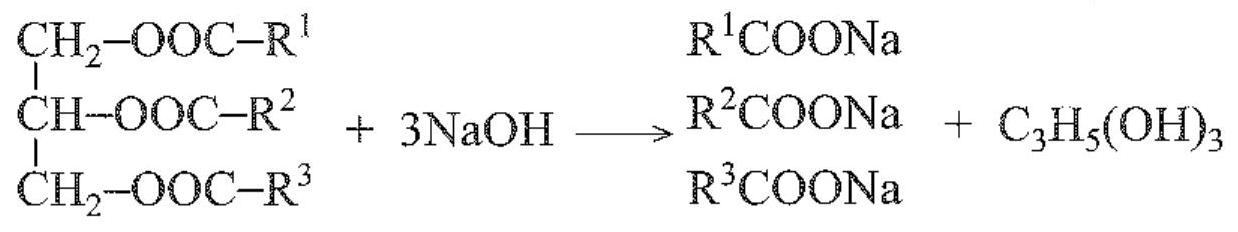
\includegraphics[max width=\textwidth, center]{2025_10_23_3f52bbaab6caa9e2ff75g-02}

Trong đó: $\mathrm{R}^{1}, \mathrm{R}^{2}$ và $\mathrm{R}^{3}$ là gốc hydrocarbon của acíd béo, chủ yếu là acid béo no.\\
2.11. a) Phản ứng với NaOH của tristearin, tripalmitin và triolein lần lượt như sau:\\
$\left(\mathrm{C}_{17} \mathrm{H}_{35} \mathrm{COO}\right)_{3} \mathrm{C}_{3} \mathrm{H}_{5}+3 \mathrm{NaOH} \rightarrow 3 \mathrm{C}_{17} \mathrm{H}_{35} \mathrm{COONa}+\mathrm{C}_{3} \mathrm{H}_{5}(\mathrm{OH})_{3}$\\
$\left(\mathrm{C}_{15} \mathrm{H}_{31} \mathrm{COO}\right)_{3} \mathrm{C}_{3} \mathrm{H}_{5}+3 \mathrm{NaOH} \rightarrow 3 \mathrm{C}_{15} \mathrm{H}_{31} \mathrm{COONa}+\mathrm{C}_{3} \mathrm{H}_{5}(\mathrm{OH})_{3}$\\
$\left(\mathrm{C}_{17} \mathrm{H}_{33} \mathrm{COO}\right)_{3} \mathrm{C}_{3} \mathrm{H}_{5}+3 \mathrm{NaOH} \rightarrow 3 \mathrm{C}_{17} \mathrm{H}_{33} \mathrm{COONa}+\mathrm{C}_{3} \mathrm{H}_{5}(\mathrm{OH})_{3}$\\
b) Ta có $\mathrm{n}_{\text {triglyceride }}=\left(\frac{300}{890}+\frac{400}{806}+\frac{300}{884}\right) \cdot 10^{3}=\mathrm{n}_{\text {glycerol } \ldots}$.

Theo phương trình ta có $\mathrm{n}_{\mathrm{NaOH}}=3 . \mathrm{n}_{\text {triglyceride }}$\\
Áp dụng định luật bảo toàn khối lượng ta có:

$$
\mathrm{m}_{\text {myối }}=\left(\mathrm{m}_{\text {triglyceride }}+\mathrm{m}_{\mathrm{NaOH}}-\mathrm{m}_{\text {glyccrol }}\right), 0,85
$$

Vậy $\mathrm{m}_{\text {muối }}=877910,809 \mathrm{~g}$ và $\mathrm{m}_{\text {xà phòng }}=1219320,569 \mathrm{~g} \approx 1,22$ (tấn).

\section*{BÀ 3}
3.1. A.\\
3.2. C.\\
3.3. C.\\
3.4. a) (1) cellulose; (2) $\beta-1,4$-glycoside.\\
b) (3) saccharose; (4) $\alpha-1,2$-glycoside.\\
3.5. C.\\
3.6. B.\\
3.7. B.\\
3.8. D.\\
3.9. C.\\
3.10. D.\\
3.11. A.\\
3.12. A.\\
3.13. A.\\
3.14. Sorbitol không phải hợp chất carbohydrate. Vì sorbitol không có công thức cấu tạo dạng $\mathrm{C}_{\mathrm{m}}\left(\mathrm{H}_{2} \mathrm{O}\right)_{\mathrm{n}}$, đồng thời sorbitol cũng không phải hợp chất tạp chức.\\
3.15. Trên phổ IR của fructose thấy xuất hiện các hấp thụ đặc trưng cho nhóm chức -OH ở vùng $3415 \mathrm{~cm}^{-1}, 3624 \mathrm{~cm}^{-1}$ nhưng không thấy hấp thụ đặc trưng của nhóm ketone ở khoảng $1750-1650 \mathrm{~cm}^{-1}$. Điều đó cho thấy nhóm chức $>\mathrm{C}=\mathrm{O}$ trong phân tử fructose đã tham gia phản ứng tạo vòng với nhóm chức- OH để tạo vòng hemiketal hay fructose không còn tồn tại ở dạng mạch hở nữa.\\
3.16. Ethanol sinh học là ethanol được sản xuất từ các nguồn nguyên liệu có nguồn gốc từ thực vật như tinh bột, cellulose,... Ở Việt Nam hiện nay, ethanol sinh học được sản xuất chủ yếu từ củ mì (củ sắn).

\section*{BÀI 4}
4.1. (1) xanh nhạt; (2) xanh lam; (3) alcohol đa chúc; (4) aldehyde.\\
4.2.B.\\
4.3. D.\\
4.4. (a) Sai; (b) Đúng; (c)\\
(d) Sai.\\
4.5. D.\\
4.6. A.\\
4.7. C.\\
4.8. C.\\
4.9. C.\\
4.10. B.\\
4.11. A.\\
4.12. B.\\
4.13. D.\\
4.14. A.\\
4.15. Quá trình lên men tạo ethanol từ glucose có sinh ra $\mathrm{CO}_{2}$ nên làm dung dịch nước vôi trong trong ống nghiệm vẩn đục. Nếu lượng $\mathrm{CO}_{2}$ quá nhiều, nước vôi có thể trong trở lại.

$$
\begin{aligned}
& \mathrm{C}_{6} \mathrm{H}_{12} \mathrm{O}_{6} \xrightarrow{\text { men }} 2 \mathrm{C}_{2} \mathrm{H}_{5} \mathrm{OH}+2 \mathrm{CO}_{2} \\
& \mathrm{CO}_{2}+\mathrm{Ca}(\mathrm{OH})_{2} \rightarrow \mathrm{CaCO}_{3}+\mathrm{H}_{2} \mathrm{O} \\
& \mathrm{CaCO}_{3}+\mathrm{H}_{2} \mathrm{O}+\mathrm{CO}_{2} \rightarrow \mathrm{Ca}\left(\mathrm{HCO}_{3}\right)_{2}
\end{aligned}
$$

4.16. Phản ứng của glucose với methanol khi có xúc tác hydrogen chloride:\\
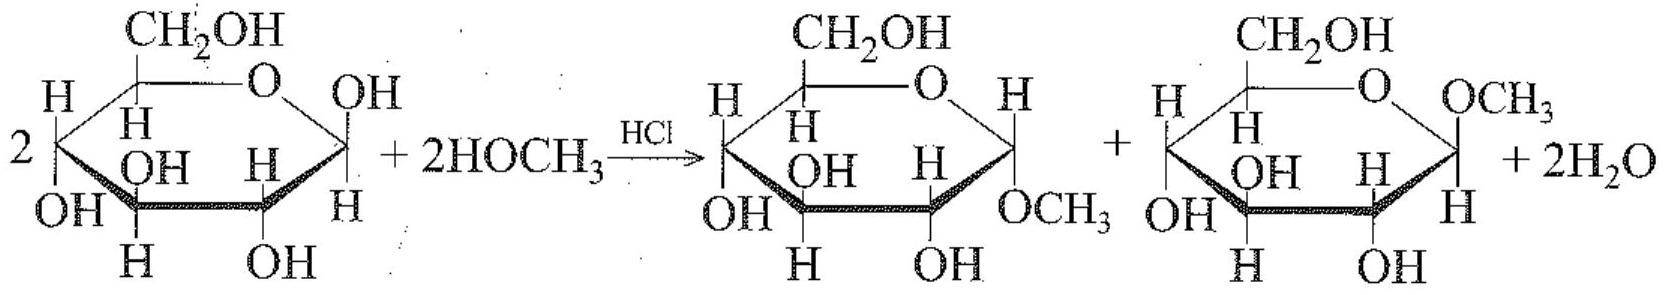
\includegraphics[max width=\textwidth, center]{2025_10_23_3f52bbaab6caa9e2ff75g-04}

Trong phản ứng trên, chỉ nhóm chức -OH hemiacetal trong phân tử glucose tham gia vào phản ứng. Glucose ở dạng mạch hở không có nhóm -OH hemiacetal nên không tham gia vào phản ứng này.\\
4.17. $\left(\mathrm{C}_{6} \mathrm{H}_{10} \mathrm{O}_{5}\right)_{\mathrm{n}}+\mathrm{nH}_{2} \mathrm{O} \xrightarrow{\mathrm{H}^{+}, \mathrm{t}^{\mathrm{c}}} \mathrm{nC}_{6} \mathrm{H}_{12} \mathrm{O}_{6}$\\
$\mathrm{C}_{6} \mathrm{H}_{12} \mathrm{O}_{6} \xrightarrow{\text { men }} 2 \mathrm{C}_{2} \mathrm{H}_{5} \mathrm{OH}+2 \mathrm{CO}_{2}$\\
$\mathrm{C}_{2} \mathrm{H}_{5} \mathrm{OH} \xrightarrow[180^{\circ} \mathrm{C}]{\mathrm{H}_{2} \mathrm{SO}_{4}} \mathrm{C}_{2} \mathrm{H}_{4}+\mathrm{H}_{2} \mathrm{O}$\\
$\mathrm{C}_{2} \mathrm{H}_{5} \mathrm{OH}+\mathrm{O}_{2} \xrightarrow{\text { men }} \mathrm{CH}_{3} \mathrm{COOH}+\mathrm{H}_{2} \mathrm{O}$\\
$2 \mathrm{CH}_{2}=\mathrm{CH}_{2}+2 \mathrm{CH}_{3} \mathrm{COOH}+\mathrm{O}_{2} \xrightarrow{\mathrm{xt}} 2 \mathrm{CH}_{3} \mathrm{COOCH}=\mathrm{CH}_{2}+2 \mathrm{H}_{2} \mathrm{O}$\\
4.18. Chất X là cellulose có công thức phân tử $\left(\mathrm{C}_{6} \mathrm{H}_{10} \mathrm{O}_{5}\right)_{\mathrm{n}}$ hay $\left[\left(\mathrm{C}_{6} \mathrm{H}_{7} \mathrm{O}_{2}(\mathrm{OH})_{3}\right]_{\mathrm{n}}\right.$. Cho chất $X$ tác dụng với hỗn hợp $\mathrm{HNO}_{3}$ và $\mathrm{H}_{2} \mathrm{SO}_{4}$ đặc sẽ tạo sản phẩm $Y$ có công thức là $\left[\left(\mathrm{C}_{6} \mathrm{H}_{7} \mathrm{O}_{2}(\mathrm{OH})_{3-\mathrm{x}}\left(\mathrm{ONO}_{2}\right)_{\mathrm{x}}\right]_{\mathrm{n}}\right.$.\\
Do hàm lượng nitrogen trong Y là $11,12 \%$ nên: $\frac{14 \mathrm{x}}{162+45 \mathrm{x}}=\frac{11,12}{100} \Rightarrow \mathrm{x}=2,0$.\\
Vậy Y có công thức $\left[\left(\mathrm{C}_{6} \mathrm{H}_{7} \mathrm{O}_{2}(\mathrm{OH})\left(\mathrm{ONO}_{2}\right)_{2}\right]_{\mathrm{n}}\right.$ và phản ứng hoá học tạo thành Y từ X như sau:\\
$\left[\mathrm{C}_{6} \mathrm{H}_{7} \mathrm{O}_{2}(\mathrm{OH})_{3}\right]_{\mathrm{n}}+2 \mathrm{nHNO}_{3} \xrightarrow{\mathrm{H}_{2} \mathrm{SO}_{4} \text { đặc }}\left[\left(\mathrm{C}_{6} \mathrm{H}_{7} \mathrm{O}_{2}(\mathrm{OH})\left(\mathrm{ONO}_{2}\right)_{2}\right]_{\mathrm{n}}+2 \mathrm{nH}_{2} \mathrm{O}\right.$\\
4.19. $\mathrm{CH}_{2} \mathrm{OH}[\mathrm{CHOH}]_{4} \mathrm{CHO}+2 \mathrm{AgNO}_{3}+3 \mathrm{NH}_{3}+\mathrm{H}_{2} \mathrm{O} \xrightarrow{t^{0}}$

$$
\mathrm{CH}_{2} \mathrm{OH}[\mathrm{CHOH}]_{4} \mathrm{COONH}_{4}+2 \mathrm{Ag}+2 \mathrm{NH}_{4} \mathrm{NO}_{3}
$$

Khối lượng bạc cần phủ trên tấm kính là: $0,72.10000=7200(\mathrm{~g})$ hay $7,2 \mathrm{~kg}$.

Khối lượng silver nitrate cần dùng là: $\frac{7,2}{108} \cdot 170 \cdot \frac{100}{90}=12,59(\mathrm{~kg})$.\\
Khối lượng glưcose cần dùng là: $\frac{7,2}{108} \cdot \frac{180}{2} \cdot \frac{100}{90}=6,67(\mathrm{~kg})$.\\
4.20*. a) Phương trình hoá học của phản úng giữa glụcose và iodine:

$$
\mathrm{CH}_{2} \mathrm{OH}[\mathrm{CHOH}]_{4} \mathrm{CHO}+\mathrm{I}_{2}+\mathrm{H}_{2} \mathrm{O} \longrightarrow \mathrm{CH}_{2} \mathrm{OH}[\mathrm{CHOH}]_{4} \mathrm{COOH}+2 \mathrm{HI}
$$

b) Chất X trong thí nghiệm trên là hồ tinh bột, có vai trò là chất chỉ thị cho phản ứng giữa iodine và sodium thiosulfate. Khi còn iodine, dung dịch có màu xanh (là màu của phức chất giữa tinh bột và iodine). Kết thúc chuẩn độ, dung dịch chuyển từ màu xanh sang không màu.\\
c) Dựa vào thể tích sodium thiosulfate tiêu tốn và nồng độ (đã biết) của dung dịch, tính được lượng sodium thiosulfate và suy ra lượng iodine còn dư sau phản ứng với glucose. Do lượng iodine ban đầu đã biết nên tính được lượng iodine đã tham gia phản ứng với glucose, từ đó tính được lượng glucose có trong mẫu.

\section*{BÀI 5}
5.1. (1) hydrogen; (2) amine; (3) hydrogen; (4) amine; (5) một; (6) base; (7) acid; (8) xanh; (9) alkyl halide.\\
5.2. D. Aniline (rất ít tan trong nước) phản ứng với HCl tạo thành muối tan tốt trong nước và bị rửa trôi.\\
5.3. B. 5.4. (a) Đúng; (b) Sai; (c) Sai; (d) Đúng.\\
5.5. D. Công thức phân tử của X là $\mathrm{C}_{7} \mathrm{H}_{9} \mathrm{~N}$.

Có 3 amine thơm bậc một ( $o-, m^{-}, p-\mathrm{CH}_{3} \mathrm{C}_{6} \mathrm{H}_{4} \mathrm{NH}_{2}$ ).\\
5.6. (a) Đúng; (b) Đúng; (c) Đúng; (d) Sai.\\
5.7. A. 5.8. B. 5.9. B.\\
5.10. (a) Đúng; (b) Sai; (c) Đúng; (d) Sai.\\
5.11. (a) Sai; (b) Đúng; (c) Sai; (d) Đúng.\\
5.12. b) Các amine bậc một là $\mathrm{C}_{4} \mathrm{H}_{9} \mathrm{NH}_{2}$, gồm 4 đồng phân cấu tạo.

Các amine bậc hai là $\mathrm{CH}_{3} \mathrm{NHC}_{3} \mathrm{H}_{7}$ (trong đó có 2 đồng phân gốc $-\mathrm{C}_{3} \mathrm{H}_{7}$ ) và $\mathrm{C}_{2} \mathrm{H}_{5} \mathrm{NHC}_{2} \mathrm{H}_{5}$.\\
Amine bậc ba là $\left(\mathrm{CH}_{3}\right)_{2} \mathrm{NC}_{2} \mathrm{H}_{5}$.\\
c) Tên theo danh pháp thay thế của các amine bậc một:\\
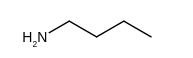
\includegraphics{smile-b806194d0918c38947b60974329d1851b913633c}

butan-1-amine\\
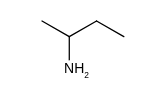
\includegraphics{smile-5b293306429e7b131bf78d38275cc8f2d82842bb}

2-methylpropan-2-amine\\
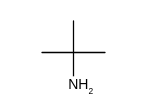
\includegraphics{smile-ab45790aa4b14dac56d44336fe7bcc7dec8a7801}\\
5.13. Phương trình hoá học của các phản ứng:\\
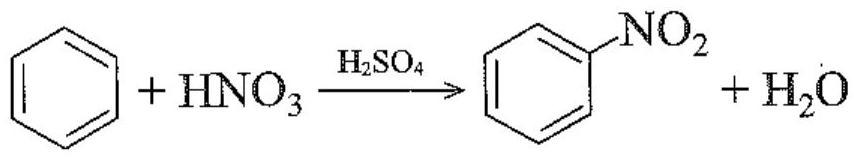
\includegraphics[max width=\textwidth, center]{2025_10_23_3f52bbaab6caa9e2ff75g-06(1)}\\
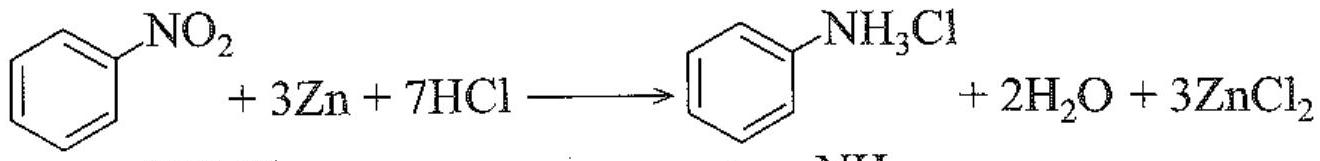
\includegraphics[max width=\textwidth, center]{2025_10_23_3f52bbaab6caa9e2ff75g-06(2)}\\
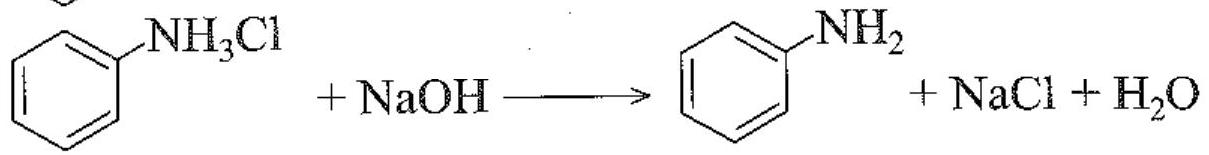
\includegraphics[max width=\textwidth, center]{2025_10_23_3f52bbaab6caa9e2ff75g-06}

\section*{BÀl 6}
6.1. D.\\
6.2. C.\\
6.3. B.\\
6.4. A.\\
6.5. D.\\
6.6. C.\\
6.7. D.\\
A. Đúng. Từ kết quả phân tích nguyên tố; lập được công thức đơn giản nhất của X là $\mathrm{C}_{4} \mathrm{H}_{9} \mathrm{O}_{2} \mathrm{~N}$. Công thức phân tử của X là: $\left(\mathrm{C}_{4} \mathrm{H}_{9} \mathrm{O}_{2} \mathrm{~N}\right)_{n}$.\\
Từ phổ MS , ta có: $\mathrm{M}_{\mathrm{X}}=103 \mathrm{n}=103 \Rightarrow \mathrm{n}=1$. Công thức phân tử của X là $\mathrm{C}_{4} \mathrm{H}_{9} \mathrm{O}_{2} \mathrm{~N}$.\\
B. Đúng. Có $2 \alpha$-amino acid: $\mathrm{NH}_{2} \mathrm{CH}\left(\mathrm{C}_{2} \mathrm{H}_{5}\right) \mathrm{COOH}$ và $\mathrm{NH}_{2} \mathrm{C}\left(\mathrm{CH}_{3}\right)_{2} \mathrm{COOH}$.\\
C. Đúng. Có các ester đồng phân với $\mathrm{X}: \mathrm{H}_{2} \mathrm{NCH}_{2} \mathrm{COOC}_{2} \mathrm{H}_{5}$, $\mathrm{H}_{2} \mathrm{NCH}_{2} \mathrm{CH}_{2} \mathrm{COOCH}_{3}, \mathrm{H}_{2} \mathrm{NCH}\left(\mathrm{CH}_{3}\right) \mathrm{COOCH}_{3}$. Trong phân tử các chất này có nhóm $-\mathrm{NH}_{2}$, nên dung dịch có tính base.\\
D. Sai. Vì X là amino acid có số nhóm $-\mathrm{NH}_{2}$ bằng số nhóm -COOH , nên ở môi trường trung tính như $\mathrm{pH}=6$ thì X ở dạng ion lưỡng cực và không bị dịch chuyển bởi điện trường.\\
6.8. D.\\
6.9. (a) Đúng; (b) Đúng; (c) Đúng; (d) Đúng.\\
(c) Có $2 \alpha$-amino acid: $\mathrm{CH}_{3} \mathrm{CH}_{2} \mathrm{CH}\left(\mathrm{NH}_{2}\right) \mathrm{COOH}$ và $\left(\mathrm{CH}_{3}\right)_{2} \mathrm{C}\left(\mathrm{NH}_{2}\right) \mathrm{COOH}$.\\
6.10. (a) Đúng; (b) Sai; (c) Sai; (d) Đúng.\\
6.11. (a) Sai; (b) Đúng; (c) Đúng; (d) Sai.\\
6.12. B.\\
6.13. Một cách gần đúng, khi trong phân tử amino acid:

\begin{itemize}
  \item Số nhóm $-\mathrm{NH}_{2}=$ số nhóm -COOH : dung dịch có môi trường trung tính.
  \item Số nhóm $-\mathrm{NH}_{2}>$ số nhóm -COOH : dung dịch có môi trường base.
  \item Số nhóm $-\mathrm{NH}_{2}$ < số nhóm -COOH : dung dịch có môi trường acid.\\
6.14. X1: methylamine; X2: hồ tinh bột; X3: glucose; X4: glycine.
\end{itemize}

\section*{BÀl 7}
\subsection*{7.1. A.}
7.2. C. Liên kết peptide là liên kết giữa nhóm $\mathrm{C}=\mathrm{O}$ của $\alpha$-amino acid này với nguyên tử N thuộc nhóm amino cúa $\alpha$-amino acid khác.\\
7.3. D.\\
7.4. B. Trong môi trường base NaOH , các amino acid tồn tại dưới dạng muối của nhóm - COOH (có nhóm - COONa ).\\
7.5. C. Chỉ các tripeptide trở lên (có từ 2 liên kết peptide trở lên) mới có phản ứng màu biuret.\\
7.6. C.\\
7.7. C. Ở nhiệt độ cao, các enzyme bị phân hủy nên mất tính xúc tác. Trong môi trường acid, các enzyme bị biến đổi cấu trúc (nhận ion $\mathrm{H}^{+}$, do các enzyme được cấu tạo từ các protein).\\
7.8. (a) Sai; (b) Đúng; (c) Sai; (d) Đúng.\\
7.9. (a) Sai; (b) Đúng; (c) Đúng; (d) Sai.\\
(d) Sai, vì chỉ đúng với các protein đơn giản; các protein phức tạp khi bị thuỷ phân còn sinh ra các thành phần khác.\\
7.10. A. Từ phần trăm khối lượng nguyên tố và phân tử khối xác định được công thức phân tử của X là $\mathrm{C}_{5} \mathrm{H}_{10} \mathrm{O}_{3} \mathrm{~N}_{2}$.\\
Vì X là dipeptide, nên X phải có 2 đon vị $\alpha$-amino acid. Vậy các $\alpha$-amino acid phải là: $\mathrm{H}_{2} \mathrm{NCH}_{2} \mathrm{COOH}$ và $\mathrm{H}_{2} \mathrm{NCH}\left(\mathrm{CH}_{3}\right) \mathrm{COOH}$. Từ đó, dipeptide X có thể là $\mathrm{H}_{2} \mathrm{NCH}_{2} \mathrm{CONHCH}\left(\mathrm{CH}_{3}\right) \mathrm{COOH}$.

\section*{BAI 8}
8.1. (1) phân tử khối; (2) mắt xích; (3) polymer; (4) hệ số polymer hoá; (5) $\mathrm{CH}_{2}=\mathrm{CH}_{2}$; (6) rắn; (7) không; (8) không tan; (9) trùng hợp; (10) trùng ngưng.\\
8.2.1-e;2-d;3-a;4-c;5-b.\\
8.3.1-d; 2-a, c; 3-b, d, e; 4-c; 5-b, e.\\
8.4. D.\\
8.5. C.\\
8.6. B.\\
8.7. D.\\
8.8. C.\\
8.9. A.\\
8.10. C.\\
8.11. (a), (b), (c).\\
8.12. (a) Sai; (b) Đúng; (c) Sai; (d) Đúng.\\
8.13. (a) Đúng; (b) Đúng; (c) Sai; (d) Đúng. 8.14. (a), (d).\\
8.15. Cellulose triacetate: $\left[\mathrm{C}_{6} \mathrm{H}_{7} \mathrm{O}_{2}\left(\mathrm{OOCCH}_{3}\right)_{3}\right]_{\mathrm{n}}$ hay $\left(\mathrm{C}_{12} \mathrm{H}_{16} \mathrm{O}_{8}\right)_{\mathrm{n}}$ có phân tử khối là 288 n. Số lượng mắt xích trong đoạn mạch CTA là $345600: 288=1200$.\\
8.16. X có công thức dạng $\left(\mathrm{C}_{\mathrm{x}} \mathrm{H}_{\mathrm{y}} \mathrm{ON}\right)_{\mathrm{n}}$.

Ta có: $\mathrm{M}_{\mathrm{x}}=(12 \mathrm{x}+\mathrm{y}+16+14) \mathrm{n}=(12 \mathrm{x}+\mathrm{y}+30) .500=56500$\\
$\Rightarrow 12 \mathrm{x}+\mathrm{y}+30=\frac{56500}{500}=113 \Rightarrow 12 \mathrm{x}+\mathrm{y}=83$\\
$\Rightarrow \mathrm{x} \leq \frac{83}{12}=6,9 \Rightarrow \mathrm{x}=6 ; \mathrm{y}=11$.\\
Vậy mắt xích của $X$ có công thức $\mathrm{C}_{6} \mathrm{H}_{11} \mathrm{ON}$ và $X$ có cấu tạo $-\left(\mathrm{NH}\left[\mathrm{CH}_{2}\right]_{5} \mathrm{CO}\right)_{n}$.

\section*{BÀl 9}
9.1. B.\\
9.2. A.\\
9.3. C.\\
9.4. B.\\
9.5. A.\\
9.6. (a), (b), (d). 9.7. (a), (b), (d).\\
9.8. 1 - a, b, c; 2 -d, g; 3-g; 4-a, b, c; 5-a, g; 6-b, c.\\
9.9. B.\\
9.10. (a), (c).\\
9.11. (b), (c), (d).\\
9.12. A.\\
9.13. C.\\
9.14. A.\\
9.15. (b), (c), (d).\\
9.16. (a), (b), (c).\\
9.17.

\begin{center}
\begin{tabular}{|l|l|l|l|}
\hline
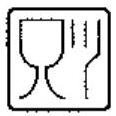
\includegraphics[max width=\textwidth]{2025_10_23_3f52bbaab6caa9e2ff75g-08(1)}
 & An toàn khi đựng thực phẩm & 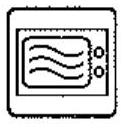
\includegraphics[max width=\textwidth]{2025_10_23_3f52bbaab6caa9e2ff75g-08}
 & Dùng được trong lò vi sóng \\
\hline
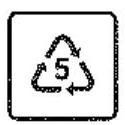
\includegraphics[max width=\textwidth]{2025_10_23_3f52bbaab6caa9e2ff75g-08(2)}
 & Chế tạo từ vật liệu polypropylene (PP) & 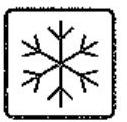
\includegraphics[max width=\textwidth]{2025_10_23_3f52bbaab6caa9e2ff75g-08(3)}
 & Sử dụng được trong tú đông \\
\hline
\end{tabular}
\end{center}

9.18. $\mathrm{C}_{2} \mathrm{H}_{4} \xrightarrow[(1)]{\mathrm{Cl}_{2}} \mathrm{ClCH}_{2} \mathrm{CH}_{2} \mathrm{Cl} \xrightarrow[(2)]{500^{\circ} \mathrm{C}} \mathrm{CH}_{2}=\mathrm{CHCl} \xrightarrow[(3)]{ }\left(\mathrm{C}_{2} \mathrm{H}_{3} \mathrm{Cl}\right)_{\mathrm{n}}$ Số kg PVC thu được là: $\frac{10^{3}}{24,79} .50 \% .65 \% .60 \% .62,5=491,63(\mathrm{~kg})$.\\
9.19. $2 \mathrm{C}_{2} \mathrm{H}_{4} \xrightarrow{+\mathrm{H}_{2} \mathrm{O}} 2 \mathrm{C}_{2} \mathrm{H}_{5} \mathrm{OH} \xrightarrow[-\mathrm{H}_{2} \mathrm{O},-\mathrm{H}_{2}]{ } \mathrm{C}_{4} \mathrm{H}_{6} \longrightarrow\left(\mathrm{C}_{4} \mathrm{H}_{6}\right)_{\mathrm{n}}$

Số $\mathrm{m}^{3}$ ethylene cần dùng là: $2 \cdot \frac{1000}{54} \cdot \frac{100}{65} \cdot \frac{100}{50} \cdot \frac{100}{70} \cdot 24,79=4036\left(\mathrm{~m}^{3}\right)$.\\
9.20. Theo sơ đồ tổng hợp caprolactam từ cyclohexanone: $\mathrm{C}_{6} \mathrm{H}_{10} \mathrm{O} \rightarrow \mathrm{C}_{6} \mathrm{H}_{11} \mathrm{ON}$.

Khối lượng cyclohexanone cần: $\frac{10}{113} \cdot 98 \cdot \frac{100}{60}=14,45$ (triệu tấn).

\section*{BÀI 10}
10.1. a) (1) nguyên tố; (2) oxi hoá - khử; (3) nhận; (4) nhường.\\
b) (1) $\mathrm{Ni}^{2+}$; (2) Zn ; (3) $\mathrm{Ni}^{2+} / \mathrm{Ni}$; (4) $\mathrm{Zn}^{2+} / \mathrm{Zn}$.\\
10.2. (b), (d).\\
10.3. a) (1) mạnh; (2) yếu; (3) nhỏ; (4) mạnh; (5) yếu.\\
b) (1) oxi hoá; (2) khử; (3) Fe; (4) $\mathrm{Cu}^{2+}$; (5) Cu ; (6) oxi hoá.\\
10.4. (a), (d).\\
(a) Sai. Vi thế điện cực chuẩn của cặp $\mathrm{Cu}^{2+} / \mathrm{Cu}$ nhỏ hơn thế điện cực chuẩn của cặp $\mathrm{Fe}^{3+} / \mathrm{Fe}^{2+}$ nên ion $\mathrm{Cu}^{2+}$ có tính oxi hoá yếu hơn ion $\mathrm{Fe}^{3+}$.\\
(d) Sai. Vì trong dãy hoạt động hoá học, kim loại đứng trước hoạt động hoá học mạnh hơn kim loại đứng sau tức là dễ bị oxi hoá hơn nên thế điện cực chuẩn phải nhỏ hơn.\\
10.5. (a), (b). 10.6. D.\\
10.7. a) $\mathrm{Cl}_{2}(g)$; b) $\mathrm{Al}(s)$; c) $\mathrm{Co}(s)$.

Chất có khả năng khử $\mathrm{Sn}^{4+}(a q)$ thành $\mathrm{Sn}^{2+}(a q)$ nhưng không khử được $\mathrm{Cr}^{3+}(a q)$ thành $\mathrm{Cr}(s)$ ở điều kiện chuẩn phải có thế điện cực chuẩn của cặp oxi hoá - khử tương ứng nhỏ hơn thế điện cực chuẩn của cặp $\mathrm{Sn}^{4+} / \mathrm{Sn}^{2+}$ và lớn hơn hơn thế điện cực chuẩn của cặp $\mathrm{Cr}^{3+} / \mathrm{Cr}$. Vậy chỉ có cặp oxi hoá khử $\mathrm{Co}^{2+} / \mathrm{Co}\left(\mathrm{E}^{0}=-0,280 \mathrm{~V}\right)$ thoả mãn điều kiện.\\
10.8. A.\\
10.9. (a), (d).\\
10.10. A.\\
10.11. B.\\
10.12. (a), (d), (e).

Khi bị ăn mòn hoặc bị gỉ, sắt kim loại bị oxi hoá thành $\mathrm{Fe}^{2+}$. Những kim loại có thể bảo vệ được Fe phải dễ bị oxi hoá hơn Fe, tức là có thế khử chuẩn nhỏ hơn thế khử chuẩn của $\mathrm{Fe}^{2+} / \mathrm{Fe} . \mathrm{Chi} \mathrm{Cr}, \mathrm{Zn}$ và Mn đáp ứng được điều kiện này.\\
10.13. $\mathrm{Al}>\mathrm{Fe}>\mathrm{Pb}>\mathrm{Cu}$.\\
10.14*. a) Dung dịch chuyển từ không màu sang màu xanh.\\
b) $\mathrm{Cu}(s)+2 \mathrm{AgNO}_{3}(a q) \rightarrow \mathrm{Cu}\left(\mathrm{NO}_{3}\right)_{2}(a q)+2 \mathrm{Ag}(s)$\\
c) $\mathrm{Cu}^{2+} / \mathrm{Cu} ; \mathrm{Ag}^{+} / \mathrm{Ag}$. Cu là tác nhân khử và $\mathrm{Ag}^{+}$là tác nhân oxi hoá.\\
d) Theo phương trình hoá học của phản ứng, lượng Cu tham gia phản ứng là:

$$
0,125.0,255.64: 2=1,02(\mathrm{~g})
$$

Vậy khối lượng thanh đồng sau khi phản ứng kết thúc là:

$$
(12,340-1,02)+(0,125 \cdot 0,255) \cdot 108=14,7625(\mathrm{~g})
$$

10.15*. a) (1) Ion $\mathrm{MnO}_{4}^{-}$có màu tím oxi hoá $\mathrm{Fe}^{2+}$ thành $\mathrm{Fe}^{3+}$ có màu vàng và nó bị khử thành ion $\mathrm{Mn}^{2+}(a q)$ không màu.\\
b) $\mathrm{MnO}_{4}^{-} / \mathrm{Mn}^{2+}$; $\mathrm{Fe}^{3+} / \mathrm{Fe}^{2+}$; thế điện cực chuẩn của cặp $\mathrm{Fe}^{3+} / \mathrm{Fe}^{2+}$ nhỏ hơn thế điện cực chuẩn của cặp $\mathrm{MnO}_{4}^{-} / \mathrm{Mn}^{2+}$.\\
c) $\mathrm{Fe}^{3+}(a q)+\mathrm{e} \rightarrow \mathrm{Fe}^{2+}(a q)$

$$
\begin{aligned}
& \mathrm{MnO}_{4}^{-}(a q)+8 \mathrm{H}^{+}(a q)+5 \mathrm{e} \rightarrow \mathrm{Mn}^{2+}(a q)+4 \mathrm{H}_{2} \mathrm{O}(l) \\
& 5 \mathrm{Fe}^{2+}(a q)+\mathrm{MnO}_{4}^{-}(a q)+8 \mathrm{H}^{+}(a q) \rightarrow \mathrm{Mn}^{2+}(a q)+5 \mathrm{Fe}^{3+}(a q)+4 \mathrm{H}_{2} \mathrm{O}(l)
\end{aligned}
$$

\section*{BÀI 11}
11.1. a) (1) hoá học; (2) điện năng.\\
b) (1) cặp oxi hoá - khử; (2) chất khử; (3) điện hoá.\\
11.2. (c), (d).\\
11.3. B.\\
11.4. D.\\
11.5. (a) Đúng; (b) Đúng; (c) Sai; (d) Sai.\\
11.6. Đây là một ví dụ sau khi đã hoàn thiện. Học sinh có thể có đáp án khác.

\begin{center}
\begin{tabular}{|l|l|l|}
\hline
Thanh phân & Vai tro & Vi du \\
\hline
Điện cực dương (cathode) & Nơi diễn ra phản úng khử & Ag \\
\hline
Diện cực âm (anode) & Nơi diễn ra phản ứng oxi hoá & Zn \\
\hline
Dung dịch chưa ion của điện cực âm & Môi trường cho phản ứng oxi hoá & Dung dịch $\mathrm{ZnSO}_{4}$ \\
\hline
Dung dịch chứa ion của điện cực dương & Môi trường cho phản ứng khử & Dung dich $\mathrm{AgNO}_{3}$ \\
\hline
Cầu muối & Kết nối hai nưa pin và duy trì tính trung hoà điện & $\mathrm{KNO}_{3}$ \\
\hline
\end{tabular}
\end{center}

11.7. B.\\
11.8. A.\\
11.9. A.\\
11.10. (a) Sai; (b) Sai; (c) Đúng; (d) Đúng.\\
11.11. a) (2); b) (1); c) (3); d) (4).\\
11.12. C.\\
11.13. (b), (c).\\
11.14*. Số mol electron tạo ra khi oxi hoá hoàn toàn 1 mol Zn thành $\mathrm{Zn}^{2+}$ là 2 mol . Vì vậy, khi oxi hoá hoàn toàn $0,1 \mathrm{~mol} \mathrm{Zn}$ sẽ tạo ra $0,2 \mathrm{~mol}$ electron.

Sử dụng công thức Faraday:

$$
Q \div n \cdot F=0,2 \cdot 96500=19300(C) .
$$

Từ đó: $\mathrm{Q}=\mathrm{I} . \mathrm{t} \Rightarrow 19300=0,02 . \mathrm{t} \Rightarrow \mathrm{t}=965000 \mathrm{~s}=268$ giờ.\\
Vậy khi điện cực kẽm hao mòn $0,1 \mathrm{~mol}$ thì sẽ thắp sáng được bóng đèn trong thòi gian 268 giờ.\\
11.15. C.\\
11.16. (a), (d).

\section*{BÀl 12}
12.1. a) (1) oxi hoá - khử; (2) dòng điện một chiều.\\
b) (1) mạnh hơn; (2) mạnh hơn; (3) mạnh; (4) tinh chế kim loại.\\
12.2. A.\\
12.3. Vì $\mathrm{Mn}^{2+}$ bị khử thành Mn nên Mn là cathode (cực âm của bình điện phân):

$$
\mathrm{Mn}^{2+}+2 \mathrm{e} \rightarrow \mathrm{Mn} \quad \mathrm{E}_{\mathrm{Mn}^{2+} / \mathrm{Mn}}^{0}=-1,18 \mathrm{~V} ;
$$

Sn bị oxi hoá thành $\mathrm{Sn}^{2+}$ nên Sn là anode (cực dương của bình điện phân):\\
$\mathrm{Sn} \rightarrow \mathrm{Sn}^{2+}+2 \mathrm{e} \quad \mathrm{E}_{\mathrm{Sn}^{2-1 / S n}}^{0}=-0,138 \mathrm{~V}$\\
Phản ứng xảy ra trong bình điện phân ngược với phản ứng tự xảy ra trong pin điện nên\\
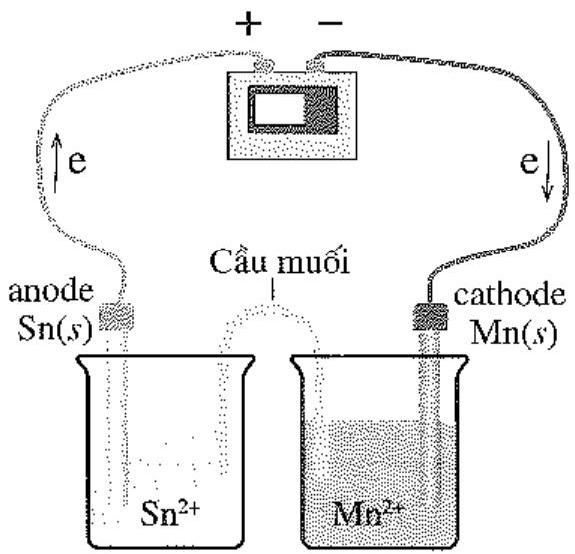
\includegraphics[max width=\textwidth, center]{2025_10_23_3f52bbaab6caa9e2ff75g-11}\\
$\mathrm{E}=\mathrm{E}_{\text {cathode }}-\mathrm{E}_{\text {anode }}=-1,18 \mathrm{~V}-(-0,138 \mathrm{~V})=-1,042 \mathrm{~V}$.\\
Vậy điện áp tối thiểu để quá trình điện phân xảy ra là $1,042 \mathrm{~V}$.\\
12.4. A. 12.5. B.\\
12.6. Khối lượng dung dịch giảm là do $\mathrm{Cl}_{2}$ và $\mathrm{H}_{2}$ bay hơi.

Đáp số: $26,856 \mathrm{~g}$.

Ở cathode (cực âm) nước bị điện phân (bị khử) : $2 \mathrm{H}_{2} \mathrm{O}+2 \mathrm{e} \rightarrow \mathrm{H}_{2}(g)+2 \mathrm{OH}^{-}$\\
Ở anode (cực dương) $\mathrm{Cl}^{-}$bị điện phân (bị oxi hoá) : $2 \mathrm{Cl}^{-} \rightarrow \mathrm{Cl}_{2}(g)+2 \mathrm{e}$\\
Gia thiết sau 2 giờ, toàn bộ NaCl bị điện phân hết, số mol electron trao đổi tại các điện cực $\mathrm{n}_{\mathrm{e}}=\frac{\mathrm{It}}{\mathrm{F}}=\frac{10.3600 .2}{96500}=0,746(\mathrm{~mol})$.\\
Vì 2 mol e được $1 \mathrm{~mol} \mathrm{Cl}_{2}$ nên số $\mathrm{mol} \mathrm{Cl}_{2}$ thoát ra tại anode là $0,373 \mathrm{~mol}$ và số $\mathrm{mol} \mathrm{H}_{2}$ thoát ra ở cathode là $0,373 \mathrm{~mol}$.\\
Khối lượng dung dịch giảm là $0,373 \cdot(2+70)=26,856(\mathrm{~g})$\\
12.7. a) Khối lượng Al trong 1000 kg quặng là 400 kg , tương ứng với khối lượng $\mathrm{Al}_{2} \mathrm{O}_{3}$ là $\frac{400}{27.2} \cdot 102=755,56(\mathrm{~kg})$.\\
Vậy \% tạp chất trong loại quặng trên là: $\frac{1000-755,56}{1000} \cdot 100 \%=24,4 \%$.\\
b) Số mol Al trong 1000 kg quặng trên là

$$
\frac{10^{3} \cdot 10^{3}}{27} \cdot 40 \%=14815(\mathrm{~mol}) .
$$

Số mol electron cần cho quá trình điện phân là:

$$
3.14815=44445(\mathrm{~mol}) \text { vì } \mathrm{Al}^{3+}+3 \mathrm{e} \rightarrow 3 \mathrm{Al} .
$$

Áp dụng công thức tính được $\mathrm{t}=119,14$ giờ.\\
12.8. A.\\
12.9. Do thế điện cực chuẩn lớn hơn nên $\mathrm{H}_{2} \mathrm{O}$ có tính oxi hoá mạnh hơn $\mathrm{Na}^{+}$, do vậy sẽ bị điện phân trước ở cathode (cực âm) theo phương trình:

$$
2 \mathrm{H}_{2} \mathrm{O}+2 \mathrm{e} \rightarrow \mathrm{H}_{2}+2 \mathrm{OH}^{-} .
$$

12.10. Dựa theo bảng thế điện cực chuẩn:

\begin{center}
\begin{tabular}{|l|c|c|c|c|}
\hline
Cặp oxi hoá/khử & $\mathrm{Fe}^{2+} / \mathrm{Fe}$ & $\mathrm{Cu}^{2+} / \mathrm{Cu}$ & $\mathrm{Ag}^{+} / \mathrm{Ag}$ & $\mathrm{Zn}^{2+} / \mathrm{Zn}$ \\
\hline
Thế điện cực chuẩn $(\mathrm{V})$ & $-0,440$ & 0,340 & 0,799 & $-0,763$ \\
\hline
\end{tabular}
\end{center}

Vì thế điện cực chuẩn càng lớn thì dạng oxi hoá có tính oxi hoá càng mạnh, do đó được điện phân trước. Vậy thứ tự điện phân ở cathode là $\mathrm{Ag}^{+}, \mathrm{Cu}^{2+}$, $\mathrm{Fe}^{2+}, \mathrm{Zn}^{2+}$.\\
12.11. Diện tích của mặt đĩa là:

$$
\mathrm{S}=\pi \mathrm{r}^{2}=\pi 12^{2}=452,16\left(\mathrm{~cm}^{2}\right)
$$

Thể tích của lớp mạ Ag cần là:

$$
V=S . d=452,16.0,001=0,45216\left(\mathrm{~cm}^{3}\right)
$$

Khối lượng Ag cần đê̂ mạ là: $\mathrm{m}=\mathrm{V} \cdot \mathrm{D}=0,45216 \cdot 10,5=4,75(\mathrm{~g})$.

Số mol Ag cần để mạ là: $\frac{4,75}{108}=0,044(\mathrm{~mol})$.\\
Từ phương trình phản ứng điện phân $\mathrm{Ag}^{+}+1 \mathrm{e} \rightarrow \mathrm{Ag}$ suy ra số mol electron cần cho điện phân lượng Ag trên là 0,044 mol.\\
Theo công thức $n(\mathrm{e})=\frac{\mathrm{It}}{\mathrm{F}}=\frac{2 \cdot 3 \cdot 60 \cdot 60}{96500}=0,2238 \mathrm{~mol}>0,044 \mathrm{~mol}$.\\
Vậy lượng điện cung cấp trong thời gian trên đủ để mạ điện chiếc đĩa nói trên.

\section*{BÀI 13}
13.1. B. Phát biểu đúng là (1), (2) và (5).\\
13.2. C.\\
13.3. (b) ${ }^{[1]}$, (c), (d).\\
(a) Sai. Vỉ ở điều kiện thường, thuỷ ngân tồn tại ở thể lỏng và không có cấu tạo tinh thể.\\
(e) Sai. Vì các electron hoá trị tự do di chuyển hỗn loạn theo nhiều hướng và không tự tạo ra dòng điện.\\
13.4. A.\\
13.5. (b), (c), (d).\\
(b) Sai. Vì nhôm được sử dụng nhiều trong chế tạo máy bay là do tính chất bền, nhẹ (khối lượng riêng nhỏ); ngoài ra tính ánh kim là do các ánh sáng nhìn thấy được bị phản xạ, không phải do các tia cực tím gây nên.\\
(c) Sai. Vì bạc có độ dẫn điện tốt nhất, nhưng do giá thành cao nên ít được sử dụng làm dây dẫn.\\
(d) Sai. Vì bạc được dùng để tráng gương là do tính ánh kim, phản xạ tốt các ánh sáng nhìn thấy được, làm hình ảnh phản chiếu rõ, sáng.\\
13.6.

\begin{center}
\begin{tabular}{|l|l|l|}
\hline
\multicolumn{1}{|c|}{Tính chát vât li} & \multicolumn{1}{c|}{\begin{tabular}{c}
Ví du ưng dung \\
tuong ung \\
\end{tabular}} & \multicolumn{1}{c|}{\begin{tabular}{c}
Vi du ki hiéu \\
loai phù hop \\
\end{tabular}} \\
\hline
Nhiệt độ nóng chảy rất cao & Dây tóc bóng đèn & W \\
\hline
Cứng & \begin{tabular}{l}
Bảo vệ bề mặt, chống \\
mài mòn \\
\end{tabular} & Cr, Nig,... \\
\hline
\end{tabular}
\end{center}

\footnotetext{[1] Trong mạng tinh thể, thời gian tồn tại của nguyên tử kim loại cực ngắn, khoảng $10^{-14}-10^{-11}$ giây.\\
Vi vậy có thể coi tinh thể kim loại M chỉ gồm các cation kim loại $\mathrm{M}^{\mathrm{n}+}$ và electron hoá trị tự do.
}\begin{center}
\begin{tabular}{|l|l|l|}
\hline
Tính chât vạt lí & V1 du úng dung turong ưng & Vi du kí hięu kim loai phù hop \\
\hline
Khối lượng riêng nhỏ & Sản xuất họp kim nhe, chế tạo máy bay,... & $\mathbf{M g}, \mathbf{A l}, \ldots$ \\
\hline
Độ dẫn điện cao & Dây dẫn điện & Cu, Al \\
\hline
Nhiệt độ nóng chảy thấp & Dây chảy của cầu chì & $\mathrm{Pb}, \mathrm{Cd}$ \\
\hline
Ánh kinn & Đồ trang sức & Ag, Au, Pt \\
\hline
\end{tabular}
\end{center}

13.7. (a) Đúng. Nhờ lực hút tĩnh điện giữa các cation kim loại và các electron hoá trị tự do mà khi bị tác dụng lực, các cation kim loại trượt lên nhau thay vì bị tách ra, làm cho kim loại có tính dẻo.\\
(b) Sai. Ở điều kiện thường, thuỷ ngân ở dạng lỏng; tuy nhiên, trong thuỷ ngân lỏng vẫn có các electron hoá trị tự do nên có thể dẫn điện được.\\
(c) Đúng. Trong thực tế, người ta dùng kim loại nhôm làm dây dẫn điện cao thế, ngoài ra còn dùng trong các thiết bị tản nhiệt, giấy gói để nướng thực phẩm.\\
(d) Sai. Tính ánh kim (vẻ ngoài lấp lánh) của kim loại là do các electron hoá trị tự do phản xạ hầu hết ánh sáng mà con người nhìn thấy được.\\
13.8. A.\\
13.9. Thứ tự dẫn điện của các kim loại giảm dần: bạc > đồng > vàng > nhôm.

Các kim loại trên đều dẫn điện tốt; tuy nhiên, do sự khác nhau về một số tính chất khác và giá thành dẫn tới phạm vi sử dụng khác nhau.

\begin{itemize}
  \item Bạc có giá thành cao nên it được sử dụng.
  \item Đồng dẫn điện tốt và rẻ hơn bạc nên được dùng làm dây dẫn điện gia đụng.
  \item Nhôm dẫn điện tốt, rẻ và nhẹ hơn các 3 kim loại còn lại rất nhiểu, phù hợp làm các dây dẫn điện cao thế có kích thước lớn.
  \item Vàng rất dẻo và bền hoá học (hầu như không bị oxi hoá) phù hợp để chế tạo các chi tiết nhỏ.
\end{itemize}

\section*{BÀI 14}
14.1. (a), (b), (d).\\
(e) sai, vì kim loại không khử kim loại mà chỉ có thể khử cation của kim loại yếu hơn trong hợp chất.\\
14.2. (a), (b), (d),\\
(c) sai, vì $\mathrm{H}_{2} \mathrm{O}$ là dạng oxi hoá với số oxi hoá của H là $+1, \mathrm{H}_{2}$ là dạng khử.\\
14.3. b), d), e).\\
14.4. (a), (c).\\
(a) sai, vì nhiều kim loại có thế khử nhỏ hơn $-0,413 \mathrm{~V}$ vẫn không phản ứng với nước ở điều kiện thường như $\mathrm{Fe}, \mathrm{Zn}$.\\
(c) sai, vì trong phản ứng giữa nước và các kim loại nhự $\mathrm{Na}, \mathrm{K}$, nước đóng vai trò là chất oxi hoá, kim loại đóng vai trò là chất khử.\\
14.5. (a) Sai, vì phản ứng tạo thành hợp chất sắt(II):

$$
\mathrm{Fe}(s)+\mathrm{Cu}^{2+}(a q) \rightarrow \mathrm{Fe}^{2+}(a q)+\mathrm{Cu}(s)
$$

(b) Đúng, màu xanh của dung dịch nhạt dần do nồng độ $\mathrm{Cu}^{2+}$ giảm dần trong phản ứng.\\
(c) Sai, tỉ lệ mol của Fe và Cu theo phản ứng là $1: 1$. Nếu 1 mol Fe tham gia phản ứng và tan ( 56 g ) sẽ có 1 mol Cu sinh ra và bám vào "đính sắt". Vì lượng kim loại tan ra nhỏ hơn lượng bám vào ( $56 \mathrm{~g}<64 \mathrm{~g}$ ) nên làm cho khối lượng của "đinh sắt" lớn hơn khối lượng của đinh sắt ban đầu.\\
(d) Sai, vì xảy ra phản ứng $\mathrm{Zn}(s)+\mathrm{Cu}^{2+}(a q) \rightarrow \mathrm{Zn}^{2+}(a q)+\mathrm{Cu}(s)$. Khi đó, nồng độ $\mathrm{Cu}^{2+}$ giảm do bị khử bởi Zn và màu xanh của dung dịch nhạt dần.\\
14.6. (a) Sai; (b) Đúng; (c) Đúng; (d) Đúng.\\
14.7. Thí nghiệm 1: $2 \mathrm{Na}+2 \mathrm{H}_{2} \mathrm{O} \rightarrow 2 \mathrm{NaOH}+\mathrm{H}_{2}$

Thí nghiệm 2: $\mathrm{Zn}+2 \mathrm{HCl} \rightarrow \mathrm{ZnCl}_{2}+\mathrm{H}_{2}$

Thí nghiệm 3: $\mathrm{Cu}+2 \mathrm{H}_{2} \mathrm{SO}_{4} \rightarrow \mathrm{CuSO}_{4}+\mathrm{SO}_{2}+2 \mathrm{H}_{2} \mathrm{O}$\\
(a) Đúng. Cả ba kim loại đều bị oxi hoá.\\
(b) Sai. Trong thí nghiệm 1, dung dịch chuyển sang màu hồng do tạo dung dịch base NaOH ; Thí nghiệm 2, dung dịch không đổi màu do dung dịch muối zinc chloride không màu; Thí nghiệm 3, dung dịch chuyển sang màu xanh do tạo thành muối copper(II) sulfate.\\
(c) Đúng. Khí $\mathbb{Z}$ là $\mathrm{SO}_{2}$, khí $\mathbb{X}$ là $\mathrm{H}_{2}$. Tỉ khối hơi $\mathrm{d}_{\mathrm{SO}_{2} / \mathrm{H}_{2}}=64 / 2=32$.\\
(d) Sai. Tổng hệ số cân bằng trong phương trình (3) bằng 7 .\\
14.8. a) Tính khử tăng dần theo dãy: $\mathrm{Hg}<\mathrm{Cu}<\mathrm{Zn}<\mathrm{K}$.\\
b) Kim loại có tính khử càng mạnh thì cation tương ứng có tính oxi hoá càng yếu. Tính oxi hoá tăng dần theo dãy: $\mathrm{K}^{+}<\mathrm{Zn}^{2+}<\mathrm{Cu}^{2+}<\mathrm{Hg}^{2+}$.\\
c) Kim loại M có giá trị thế điện cực chuẩn $\mathrm{E}_{\mathrm{M}^{\mathrm{p}} / \mathrm{M}}^{\circ}$ âm có thể tác dụng với hydrochloric acid ở điều kiện thường: $\mathrm{Zn}, \mathrm{K}$.\\
Tuy nhiên KHÔNG cho trực tiếp potassium vào dung dịch acid vì phản ứng xảy ra rất mãnh liệt và gây nổ.\\
14.9. B.\\
14.10. a) Không xảy ra phản ứng.\\
b) $\mathrm{Zn}+2 \mathrm{AgNO}_{3} \rightarrow \mathrm{Zn}\left(\mathrm{NO}_{3}\right)_{2}+2 \mathrm{Ag}$.\\
c) $2 \mathrm{Na}+2 \mathrm{H}_{2} \mathrm{O} \rightarrow 2 \mathrm{NaOH}+\mathrm{H}_{2}$.

$$
2 \mathrm{NaOH}+\mathrm{CuSO}_{4} \rightarrow \mathrm{Cu}(\mathrm{OH})_{2}+\mathrm{Na}_{2} \mathrm{SO}_{4} .
$$

d) $\mathrm{Hg}+\mathrm{S} \rightarrow \mathrm{HgS}$.\\
e) $\mathrm{Mg}+2 \mathrm{H}_{2} \mathrm{O} \rightarrow \mathrm{Mg}(\mathrm{OH})_{2}+\mathrm{H}_{2}$.\\
14.11. Do vàng có độ hoạt động hoá học yếu, có thế điện cực chuẩn lớn. Học sinh có thể tìm kiếm nhiệt tạo thành của $\mathrm{Au}_{2} \mathrm{O}_{3}$ để có thêm thông tin "quá trình hình thành $\mathrm{Au}_{2} \mathrm{O}_{3}$ không thuận lợi về mặt năng lượng".

\section*{BÀI 15}
15.1. A. 15.2. D. 15.3. A. 15.4. C.\\
15.5. Nhiệt luyện: $\mathrm{Fe}, \mathrm{Sn}, \mathrm{Zn}, \mathrm{Cu}$.

Thuỷ luyện: $\mathrm{Cu}, \mathrm{Ag}$.\\
Điện phận nóng chảy: $\mathrm{Al}, \mathrm{Na}, \mathrm{Mg}$.\\
15.6. Trong phản ứng tách kim loại từ ZnO bằng C theo phương pháp nhiệt luyện, kẽm sinh ra ở thể hơi, do nhiệt độ phản ứng cao hơn nhiệt độ hoá hơi của kẽm.\\
15.7*. Muối HgS dễ bị phân huỷ, cháy khi đun nóng hoặc tiếp xúc với lửa, sinh ra hơi thuỷ ngân rất độc. Trong thực tế, trước đây người ta dùng đá chu sa như một nguồn chủ yếu để sản xuất kim loại thuỷ ngân, người ta đốt cháy chu sa trong ống kín, ngưng tụ sản phẩm cháy thu được thuỷ ngân dạng lỏng.

$$
\begin{aligned}
& \mathrm{HgS}(s) \rightarrow \mathrm{Hg}(g)+\mathrm{S}(s) \\
& \mathrm{HgS}(s)+\mathrm{O}_{2}(g) \rightarrow \mathrm{Hg}(g)+\mathrm{SO}_{2}(g)
\end{aligned}
$$

15.8. (a) Đúng. Tại cathode $(-): \mathrm{Al}^{3+}(l)+3 \mathrm{e} \rightarrow \mathrm{Al}(l)$, theo hình vẽ, lớp nhôm nóng chảy thu được tại cực âm (phần đáy của bể điện phân).\\
(b) Đúng. Cryolite làm giảm sâu nhiệt độ nóng chảy, từ đó giảm lượng năng lượng cần cung cấp để nấu chảy hỗn hợp; ngoài ra, việc tăng độ dẫn điện còn làm tăng hiệu suất của quá trình điện phân. Do đó, làm giảm chi phí sản xuất.\\
(c) Sai. Tại anode, graphite bị ăn mòn do phản ứng với oxygen tạo thành các oxide của carbon thoát ra cùng với oxygen.

$$
\begin{gathered}
\mathrm{C}(s)+\mathrm{O}_{2}(g) \rightarrow \mathrm{CO}_{2}(g) \\
\mathrm{C}(s)+\mathrm{CO}_{2}(g) \rightarrow 2 \mathrm{CO}(g)
\end{gathered}
$$

(d) Sai. Việc thiết kế cathode bên dưới bể điện phân giứp nhôm nóng chảy sinh ra ở đáy bể tránh tiếp xúc với oxygen trong không khí, ngoài ra đi trọng của nhôm lỏng lớn hơn hỗn hợp điện phân giúp phôm lỏng chìm xuống đáy bể, không ảnh hưởng đến quá trình điện phân. Anode ở phía trên dễ dàng nhúng xuống bể liên tục kbi bị ăn mòn (việc này gần như không thể thực hiện nếu đặt anode ở đáy bể). Bên cạnh đó, nếu anode ở đáy-bể, các khí sinh ra tại anode sẽ thoát vào hỗn hợp lỏng, ảnh hưởng đến quá trình điện phân.

\section*{BÀI 16}
16.1.1-c; 2 -c; $3-a ; 4-b ; 5-c ; 6-d$.\\
16.2. (a), (c), (d), (e).\\
(b) Sai. Ví nhiệt độ nóng chảy của hợp kim $\mathbf{A - B}$ có thể cao hơn hoặc thấp hơn hẳn nhiệt độ nóng chảy của từng kim loại thành phần. Ví dụ thiếc chảy ( $\mathrm{Sn}-\mathrm{Pb}$ tỉ 1ệ $63 / 37$ ) nóng chảy ở $188^{\circ} \mathrm{C}$, thấp hơn nhiều so với nhiệt độ nóng chảy của Sn và Pb lần lượng là $232^{\circ} \mathrm{C}$ và $327^{\circ} \mathrm{C}$ nên được dùng làm hợp kim hàn.\\
16.3. C.\\
16.4. B. (1) Đúng. Vì vị trí đóng đinh thép bị ăn mòn trước là do việc đóng đinh tạo ra lồ thủng trên tấm tôn làm cho lõi thép và lớp trảng kẽm cùng tiếp xúc với không khí ẩm, nước mưa. Trong điều kiện này, vị trí đóng đinh thép sẽ xuất hiện một pin điện hoá và sự ăn mòn điện hoá diễn ra nhanh hơn so với các vị trí khác trên tấm tôn.\\
(2) Sai.\\
(3) Sai, vì ngoài sắt trong thép còn có carbon, khi hai thành phần này cùng tiếp xúc nước mưa (tại vị trí không có kêm hoặc khi lớp kẽm đã bị ăn mòn), sắt đóng vai trò là anode và vẫn bị ăn mòn.\\
(4) Đúng, vì kẽm sẽ bị ăn mòn trước.\\
16.5. Phương trình hoá học: $4 \mathrm{Ag}+\mathrm{O}_{2}+2 \mathrm{H}_{2} \mathrm{~S} \rightarrow 2 \mathrm{Ag}_{2} \mathrm{~S}+2 \mathrm{H}_{2} \mathrm{O}$

Trong trường hợp này, bạc bị ăn mòn hoá học do bạc phản ứng trực tiếp với oxygen và hydrogen sulfide, trong đó oxygen đóng vai trò là chất oxi hoá.\\
16.6. (c), (d).\\
16.7. A.\\
16.8. Vỏ tàu làm bằng thép có thành phần $\mathrm{Fe}-\mathrm{C}$, khi nhúng trong nước biển (môi trường điện li), Fe đóng vai trò là anode và bị ăn mòn. Tuy nhiên, khi gắn các khối kẽm lên vỏ tàu, do Zn có thế điện cực chuẩn âm hơn của Fe nên lúc này, Zn đóng vai trò là anode và bị ăn mòn trước Fe . Vì vậy, tấm Zn được gọi là\\
anode hi sinh. Sau một thời gian, người ta cần thay thế hoặc bổ sung các khối kẽm đã bị ăn mòn bằng các khối kẽm mới. Mặc dù vậy, việc này dễ dàng và ít chi phí hơn nhiều so với việc phải sửa chữa, gia cố vỏ tàu.\\
Bên cạnh bảo vệ vỏ tàu biển, phương pháp này còn được dùng rộng rãi trong việc bảo vệ các thiết bị, công trình làm bằng thép khó tiếp cận khác như ống dẫn dầu (chìm trong đất, dưới biển), giàn khoan, trụ điện cao thế,...\\
16.9. a) Không có ăn mòn điện hoá.\\
b) $\mathrm{Zn}(s)+2 \mathrm{Ag}^{+}(a q) \rightarrow \mathrm{Zn}^{2+}(a q)+2 \mathrm{Ag}(s)$

Bạc sinh ra (ở cathode) bám trên thanh kẽm (ở anođe), cùng tiếp xúc với dung dịch chất điện li nên xảy ra ăn mòn điện hoá.\\
c) $\mathrm{Fe}(s)+2 \mathrm{Fe}^{3+}(a q) \rightarrow 3 \mathrm{Fe}^{2+}(a q)$, không có cặp hai kim loại hay kim loại phi kim nên không xảy ra ăn mòn điện hoá.\\
d) Mg đóng vai trò là anode, Fe đóng vai trò là cathode, nước hoà tan NaCl tạo thành đung dịch chất điện li, nên xảy ra ăn mòn điện hoá.\\
e) Ở dạng rắn, hai chất không phản ứng với nhau, không đủ điều kiện xảy ra ăn mòn điện hoá.\\
16.10. a) D. Sau bước 2, hai kim loại không tiếp xúc, không được nối bằng dây dẫn nên không đủ điều kiện xảy ra ăn mòn điện hoá, hơn nữa cả hai kim loại đều không phản ứng trực tiếp với dung dịch NaCl (không có ăn mòn hoá học) nên cả hai kim loại đều không bị ăn mòn.\\
b) (2), (5).\\
c) B.

Sau bước 3, ăn mòn điện hoá diễn ra:\\
Thanh kẽm (anode): $\mathrm{Zn} \rightarrow \mathrm{Zn}^{2+}+2 \mathrm{e}$\\
Thanh đồng (cathode):

$$
\mathrm{O}_{2}+4 \mathrm{e}+2 \mathrm{H}_{2} \mathrm{O} \rightarrow 4 \mathrm{OH}^{-} \text {hoặc } 2 \mathrm{H}_{2} \mathrm{O}+2 \mathrm{e} \rightarrow 2 \mathrm{OH}^{-}+\mathrm{H}_{2} .
$$

(làm phenolphthalein chuyển sang màu hồng)

\section*{BÀ 17}
17.1.B.\\
17.2. (a), (c), (e).\\
17.3. (a), (d).\\
17.4. (b), (c), (d), (e).\\
17.5. a) $135,61 \mathrm{~kJ} \mathrm{~mol}^{-1}$.\\
b) Không thuận lợi về mặt năng lượng do là phản ứng thu nhiệt.\\
c) Có thể dựa vào giá trị biến thiên enthalpy chuẩn của phản ứng nhiệt phân trên. Phản ứng thu nhiệt nên cần cung cấp năng lượng (đưn nóng) thì phản ứng mói xảy ra.\\
17.6.C.\\
17.7. A.\\
17.8. $2 \mathrm{Na}(s)+2 \mathrm{H}_{2} \mathrm{O}(l) \rightarrow 2 \mathrm{NaOH}(a q)+\mathrm{H}_{2}(g)$\\
(a) Sai. Sodium bị hoà tan là do phản ứng trực tiếp với nước (có thể xem là ăn mòn hoá học).\\
(b) Đúng. Vì phản ứng sinh ra NaOH tạo môi trường base.\\
(c) Đúng. Khí thoát ra là hydrogen, rất dễ cháy.\\
(d) Đúng. Lithium có tính khử yếu hơn sodium và cũng phản ứng với nước chậm hơn so với sodium.\\
17.9. (a) Đúng; (b) Đúng; (c) Sai; (d) Sai.\\
17.10. B. Potassium là kim loại hoạt động hơn sodium và lithium; chlorine hoạt động hơn bromine. Trong thực tế, phản ứng giữa potassium và chlorine xảy ra dễ dàng ngay khi tiếp xúc ở điều kiện thường mà không cần phải đun nóng hay thêm xúc tác.\\
17.11*. B. Dung dịch X cháy với ngọn lửa vàng nên có chứa cation $\mathrm{Na}^{+}$; phản ứng với $\mathrm{AgNO}_{3}$ tạo kết tủa vàng, có thể chứa anion $\mathrm{I}^{-}$(tạo AgI ) hoặc $\mathrm{PO}_{4}^{3-}$ (tạo $\mathrm{Ag}_{3} \mathrm{PO}_{4}$ ).\\
17.12. Học sinh tự viết các phương trình hoá học.

Hoà tan NaCl vào nước tạo môi trường pH có giá trị khoảng 7 .\\
Hoà tan $\mathrm{Na}_{2} \mathrm{O}$ vào nước tạo môi trường base $\mathrm{pH}>7$ :

$$
\mathrm{Na}_{2} \mathrm{O}+\mathrm{H}_{2} \mathrm{O} \rightarrow 2 \mathrm{NaOH}
$$

$\mathrm{Na}_{2} \mathrm{~S}$ hoà tan vào nước tạo dung dịch có tính base $\mathrm{pH}>7$, do anion $\mathrm{S}^{2-}$ bị thuỷ phân tạo môi trường base:

$$
\mathrm{S}^{2-}+\mathrm{H}_{2} \mathrm{O} \rightleftharpoons \mathrm{HS}^{-}+\mathrm{OH}^{-}
$$

17.13. (a) Sai. Tại anode, anion chloride bị oxi hoá thành khí chlorine:

$$
2 \mathrm{Cl}^{-} \rightarrow \mathrm{Cl}_{2}+2 \mathrm{e}
$$

(b) Sai. Trong thực tế, dung dịch thu được tại cathode cần cô đặc nhiều lần để sodium hydroxide kết tinh.\\
(c) Đúng. Màng ngăn xốp giúp ngăn anion $\mathrm{OH}^{-}$di chuyển sang anode phản ứng với chlorine tạo thành nước Javel. Nếu không có màng ngăn:

$$
2 \mathrm{OH}^{-}+\mathrm{Cl}_{2} \rightarrow \mathrm{ClO}^{-}+\mathrm{Cl}^{-}+\mathrm{H}_{2} \mathrm{O}
$$

(d) Đúng. Hydrogen thu được đừ quá trình này được dùng để sản xuất hydrochloric acid, ammonia,...\\
17.14. Do thế khử chuẩn của nước (môi trường acid) xấp xỉ thế khử chuẩn của chlorine, nên khi nồng độ chloride giảm (trong nước muối nghèo) xảy ra phản ứng oxi hoá nước tại anode: $2 \mathrm{H}_{2} \mathrm{O} \rightarrow \mathrm{O}_{2}+4 \mathrm{H}^{+}+4 \mathrm{e}$, cạnh tranh với phản ứng oxi hoá anion chloride làm giảm hiệu suất điện phân; đồng thời khí chlorine thu được sẽ bị lẫn khí oxygen. Do đó, dung dịch sodium chloride tại anode cần được "làm giàu" liên tục nhằm duy trì nồng độ bão hoà NaCl . Khối lượng sodium hydroxide thu được ứng với mỗi lít nước muối bão hoà bị điện phân là: $\mathrm{m}=\frac{300-220}{58,5} \cdot 40 \cdot 0,8=43,8(\mathrm{~g})$.\\
17.15. A.\\
17.16. (b), (c), (d).\\
17.17. (a), (d).\\
(d) sai. Vì khối lượng chất rắn giảm $\frac{44+18}{2.84} \cdot 100 \%=37 \%$.\\
17.18. (a) Sai; (b) Sai; (c) Đúng; (d) Đúng.

\section*{BÀI 18}
18.1.C. 18.2. (c), (e). 18.3.C. 18.4.D.\\
18.5. a) $\mathrm{K}_{2} \mathrm{CO}_{3}(a q)+\mathrm{Ca}(\mathrm{OH})_{2}(a q) \rightarrow \mathrm{CaCO}_{3}(s)+2 \mathrm{KOH}(a q)$\\
b) $2 \mathrm{Na}_{3} \mathrm{PO}_{4}(a q)+3 \mathrm{BaCl}_{2}(a q) \rightarrow \mathrm{Ba}_{3}\left(\mathrm{PO}_{4}\right)_{2}(s)+6 \mathrm{NaCl}(a q)$\\
c) $\mathrm{Mg}\left(\mathrm{HCO}_{3}\right)_{2}(a q)+\mathrm{H}_{2} \mathrm{SO}_{4}(a q) \rightarrow \mathrm{MgSO}_{4}(a q)+2 \mathrm{CO}_{2}(g)+2 \mathrm{H}_{2} \mathrm{O}(l)$\\
d) $2 \mathrm{NaHCO}_{3}(a q)+\mathrm{Ba}(\mathrm{OH})_{2}(a q) \rightarrow \mathrm{BaCO}_{3}(s)+\mathrm{Na}_{2} \mathrm{CO}_{3}(a q)+2 \mathrm{H}_{2} \mathrm{O}(l)$\\
e) $\mathrm{Ba}(\mathrm{OH})_{2}(a q)+2 \mathrm{HNO}_{3}(a q) \rightarrow \mathrm{Ba}\left(\mathrm{NO}_{3}\right)_{2}(a q)+2 \mathrm{H}_{2} \mathrm{O}(l)$\\
18.6. (a), (b), (d), (e).\\
18.7. Học sinh tự trả lời. Lưu ý: ngoài việc bổ sung calcium cho cơ thể bằng cách ăn các thực phẩm chứa nhiều calcium phù hợp, cơ thể cũng cần tổng hợp/ bổ sung đủ lượng vitamin D để việc chuyển hoá calcium được hiệu quả.\\
18.8. (a) Đúng; (b) Đúng; (d) Đúng.\\
(c) Sai. Vì chất $\mathbb{Y}$ có thể là potassium sulfite hoặc potassium phosphate.\\
18.9. B.\\
18.10. (b), (c), (d).\\
18.11. (a) Sai.\\
(b) Đúng. Xét cân bằng: $\mathrm{BeCO}_{3}(s) \rightleftharpoons \mathrm{BeO}(s)+\mathrm{CO}_{2}(g)$, việc bảo quản $\mathrm{BeCO}_{3}(s)$ trong khí $\mathrm{CO}_{2}$ làm cân bằng dịch chuyển sang chiều nghịch, giúp làm giảm sự phân huỷ của $\mathrm{BeCO}_{3}(s)$.\\
(c) Sai. Với cùng điện tích, $\mathrm{Be}^{2+}$ có bán kính nhỏ hơn $\mathrm{Ca}^{2+}$ nên $\mathrm{Be}^{2+}$ có mật độ điện tích lớn hơn, nên dễ bị thuỷ phân hơn $\mathrm{Ca}^{2+}$...\\
(d) Đúng. Cation $\mathrm{Be}^{2+}$ có thể thay thế nguyên tử trung tâm magnesium của các phức chất trong các enzyme, qua đó làm biến đồi (ức chế) chức năng của các enzyme này và gây bệnh.\\
Trong thực tế, các công nhân làm việc trong các ngành luyện kim, tái chế kim loại, điện tử, chế tạo máy bay, tàu vũ trụ,... có thể bị phơi nhiễm beryllium dẫn tới việc họ có thể mắc một số bệnh cấp tính hoặc mạn tính gọi chung là bệnh beryllium.\\
18.12. c) Đặt m là khối lượng tinh thể $\mathrm{Ba}\left(\mathrm{NO}_{3}\right)_{2} \cdot 6 \mathrm{H}_{2} \mathrm{O}$ kết tinh.

Với nồng độ phần trăm dung dịch sau kết tinh ở $10^{\circ} \mathrm{C}$ :

$$
\mathrm{C}=\frac{6,67}{6,67+100} \cdot 100=\frac{9,02-\frac{\mathrm{m}}{369} \cdot 261}{100+9,02-\mathrm{m}} \cdot 100 \Rightarrow \mathrm{~m}=3,42 \mathrm{~g}
$$

18.13. a) Biến thiên enthalpy chuẩn của phản úng ở $25^{\circ} \mathrm{C}$ :\\
$\Delta_{\mathrm{r}} \mathrm{H}_{298}^{\mathrm{o}}=\Delta_{\mathrm{r}} \mathrm{H}_{298}^{\mathrm{o}}\left(\mathrm{Mg}(\mathrm{OH})_{2}, s\right)-\Delta_{\mathrm{f}} \mathrm{H}_{298}^{\mathrm{o}}\left(\mathrm{H}_{2} \mathrm{O}, l\right)=-928,4-(-285,8)=-642,6 \mathrm{~kJ} \mathrm{~mol}^{-1}$.\\
Lượng nhiệt tối đa toả ra bởi 1 gói FRH là: $\mathrm{Q}=\frac{8.0,9}{24} \cdot 642,6=192,78(\mathrm{~kJ})$.\\
Nhiệt lượng cần để làm nóng gói súp từ $30^{\circ} \mathrm{C}$ lên $100^{\circ} \mathrm{C}$ là:\\
$\mathrm{Q}^{\prime}=300 .(100-30) .4,2=88200(\mathrm{~J})=88,2 \mathrm{~kJ}<192,78.0,5=96,39(\mathrm{~kJ})$. Như vậy, lượng nhiệt từ 1 gói FRH có khối lượng 8 g có thể làm nóng lượng súp nói trên.\\
b) Khi cho nước vào hỗn hợp bột $\mathrm{FRH}, \mathrm{NaCl}$ bị hoà tan, tạo môi trường chất điện li, bột Mg được trộn với bột Fe trong môi trường điện li tạo thành vô số pin điện hoá với Mg là cực âm và Fe là cực dương, lúc này Mg sẽ bị oxi hoá nhanh theo cơ chế ăn mòn điện hoá:\\
Tại cực âm: $\mathrm{Mg} \rightarrow \mathrm{Mg}^{2+}+2 \mathrm{e}$\\
Tại cực dương: $2 \mathrm{H}_{2} \mathrm{O}+2 \mathrm{e} \rightarrow 2 \mathrm{OH}^{-}+\mathrm{H}_{2}$\\
c) Lượng nước thêm vào nhằm mục đích hoà tan chất điện li NaCl , đồng thời đóng vai trò như chất oxi hoá; tuy nhiên, nếu thêm nhiều nước, nước có nhiệt dung rất lớn (khoảng $4,2 \mathrm{~J} \mathrm{~g}^{-1} \mathrm{C}^{-1}$ ) nên chính lượng nước này sẽ hấp thu phần lớn lượng nhiệt toả ra, làm giảm hiệu quả đun nóng của gói FRH.

\section*{BÀI 19}
19.1. (c), (e). 19.2. (a), (c), (e). 19.3. A. 19.4. (b), (d), (e).\\
19.5. Tính cứng tạm thời của nước cứng gây nên bởi các muối $\mathrm{Ca}\left(\mathrm{HCO}_{3}\right)_{2}$ và $\mathrm{Mg}\left(\mathrm{HCO}_{3}\right)_{2}$. Khi dùng $\mathrm{Ca}(\mathrm{OH})_{2}$ với lượng vừa đủ thì các ion $\mathrm{Ca}^{2+}$ và $\mathrm{Mg}^{2+}$ bị loại bỏ gần như hoàn toàn, làm mất tính cứng của nước. Tuy nhiên, nếu dùng với lượng dư, lượng $\mathrm{Ca}^{2+}$ dư trong $\mathrm{Ca}(\mathrm{OH})_{2}$ làm nước cứng trở lại.\\
$\mathrm{Ca}\left(\mathrm{HCO}_{3}\right)_{2}(a q)+\mathrm{Ca}(\mathrm{OH})_{2}(a q) \rightarrow 2 \mathrm{CaCO}_{3}(s)+2 \mathrm{H}_{2} \mathrm{O}(l)$\\
$\mathrm{Mg}\left(\mathrm{HCO}_{3}\right)_{2}(a q)+\mathrm{Ca}(\mathrm{OH})_{2}(a q) \rightarrow \mathrm{CaCO}_{3}(s)+\mathrm{MgCO}_{3}(s)+2 \mathrm{H}_{2} \mathrm{O}(l)$.\\
19.6. Nước có tính cứng tạm thời: (1), (2), (3), (4), (5), (6).

Nước có tính cứng toàn phần: (1), (2), (3), (5), (6).\\
Nước có tính cứng vĩnh cưu: (1), (2), (5), (6).\\
19.7. a) Dung dịch trung hoà điện nên ta có:

$$
1,2.1+3,0.2+1,0.2=0,6.1+0,1.2+x .1 \Rightarrow x=8,4 \mathrm{mM}
$$

Do nồng độ của $\mathrm{HCO}_{3}^{-}>2$. (nồng độ của $\mathrm{Ca}^{2+}+$ nồng độ của $\mathrm{Mg}^{2+}$ ) nên có thể làm mất tính cứng của loại nước này khi đun sôi.\\
b) Khi đun sôi kĩ, xảy ra các phản ứng hoá học sau:

$$
\begin{aligned}
& 2 \mathrm{HCO}_{3}^{-}(a q) \xrightarrow{\mathrm{t}^{\circ}} \mathrm{CO}_{3}^{2-}(a q)+\mathrm{CO}_{2}(g)+\mathrm{H}_{2} \mathrm{O}(l) \\
& 8,4 \mathrm{mM} \quad 4,2 \mathrm{mM} \\
& \mathrm{Mg}^{2+}(a q)+\mathrm{CO}_{3}^{2-}(a q) \longrightarrow \mathrm{MgCO}_{3}(s) \\
& 1,0 \mathrm{mM} \quad 1,0 \mathrm{mM} \\
& \mathrm{Ca}^{2+}(a q)+\mathrm{CO}_{3}^{2-}(a q) \longrightarrow \mathrm{CaCO}_{3}(s) \\
& 3,0 \mathrm{mM} \quad 3,0 \mathrm{mM}
\end{aligned}
$$

Dung dịch sau đun sôi kĩ 2 lít nước cứng gồm: $2,4 \mathrm{mmol} \mathrm{Na}{ }^{+} ; 1,2 \mathrm{mmol} \mathrm{Cl}$; $0,2 \mathrm{mmol} \mathrm{SO}{ }_{4}^{2-}$ và $0,4 \mathrm{mmol} \mathrm{CO}_{3}^{2-}$.\\
Tổng khối lượng chất tan còn lại trong dung dịch:

$$
2,4.23+1,2.35,5+0,2.96+0,4.60=141(\mathrm{mg}) .
$$

\section*{BÀl 20}
20.1. B. 20.2. A. 20.3. A.\\
20.4. (a) Đúng; (b) Sai; (c) Sai; (d) Đúng.\\
20.5. (a) Đúng; (b) Sai; (c) Đúng; (d) Sai. 20.6. (a), (b).\\
20.7. 8 electron. Electron hoá trị là những electron mà nguyên tử có thể dùng để tạo liên kết hoá học. Thường bao gồm các electron ở lớp ngoài cùng và các electron ở phân lớp d chưa bão hoà.\\
20.8. 3 electron độc thân. 20.9. a) 8 mol. b2) 8 electron.\\
20.10. Học sinh tự giải thích. 20.11. (b), (c), (d), (e).\\
20.12. a) và b) dựa vào màu sắc đặc trưng của chất.\\
c) và d) dựa vào màu sắc của dung dịch trước phản ứng và màu sắc của kết tủa hình thành sau phản ứng.\\
20.13. (a) Sai\\
$5 \mathrm{Fe}^{2+}(a q)+\mathrm{MnO}_{4}^{-}(a q)+8 \mathrm{H}^{+}(a q) \rightarrow 5 \mathrm{Fe}^{3+}(a q)+\mathrm{Mn}^{2+}(a q)+4 \mathrm{H}_{2} \mathrm{O}(l)$\\
Số mol anion $\mathrm{MnO}_{4}^{-}$là:

$$
\mathrm{n}_{\mathrm{MnO}_{4}^{-}}=\mathrm{n}_{\mathrm{KMnO}_{4}}=0,040 \cdot 0,0235=0,00094(\mathrm{~mol}) .
$$

Từ phương trình hoá học: $\mathrm{n}_{\mathrm{Fe}^{21}}=5 \mathrm{n}_{\mathrm{MnO}_{4}^{-}}=5.0,00094=0,00470(\mathrm{~mol})$.\\
Khối lượng sắt trong mẫu khoáng vật bằng khối lượng $\mathrm{Fe}^{2+}$ đã phản ứng với thuốc tím và là: $0,00470.56=0,2632(\mathrm{~g})$.\\
Phần trăm theo khối lượng của Fe trong mẫu khoáng vật là:

$$
\frac{0,2632}{0,422} \cdot 100 \%=62,37 \%
$$

(b) Đúng; (c) Sai; (d) Sai (cần lặp lại thí nghiệm ít nhất 3 lần).\\
20.14. (a) Sai (dựa vào thế điện cực của cặp oxi hoá - khử để so sánh).\\
(b) Đúng (vì chỉ có $\mathrm{Fe}^{2+}$ trong dung dịch tác dụng với thuốc tím).\\
(c) Sai (trong môi trường acid, $\mathrm{Cr}_{2} \mathrm{O}_{7}^{2-}$ là chất oxi hoá khá mạnh và có màu).\\
(d) Sai (chiều của phản ứng được xác định theo thế điện cực).\\
20.15. (a), (d), (e).

\section*{BÀI 21}
21.1.C.\\
21.2. B.\\
21.3. D.\\
21.4.C.\\
21.5. (c), (d).

Có phức chất mà nguyên tử trung tâm là nguyên tố $\mathrm{s}, \mathrm{p}$.\\
Phức chất $\left[\mathrm{Ni}(\mathrm{CO})_{4}\right]$ hình thành từ quá trình nguyên tử Ni nhận các cặp electron hoá trị riêng của 4 phân tử CO .\\
21.6. (b), (c), (d).

Phân tử $\mathrm{H}_{2}$ không có cặp electron hoá trị riêng nên không thể trở thành phối tử. Không phải trong mọi trường hợp ethylenediamine đều sử dụng cả hai cặp electron để hình thành liên kết cho - nhận với nguyên tử trung tâm.\\
21.7. (a), (c), (d),\\
21.8. (a), (b), (d).

Với nguyên tử trung tâm trong phức chất: hoá trị và số phối trí thường không đồng nhất.\\
21.9. (a), (b).\\
21.10. (a) Sai. Nguyên tử trung tâm không chỉ là nguyên tố kim loại chuyển tiếp.\\
(b) Sai.\\
(c) Đúng. Do số liên kết $\sigma$ giữa nguyên tử trung tâm và phối đử ở hai phức chất khác nhau.\\
(d) Sai. Ở B chỉ có một loại phối tử.\\
21.11.1-b, d, e; 2-a, d; 3-a, c, g.\\
21.12. a) 2 .\\
b) Không. Có phức chất mà trong đó ethylenediamine chỉ sử dụng một cặp electron hoá trị riêng để tạo một liên kết cho - nhận.\\
Số cặp electron hoá trị riêng của các phân tử hoặc anion thường chỉ cho biết liên kết cho - nhận mà phân tử hoặc anion đó có khả năng tạo thành, còn số liên kết trong thực tế phải được xác định từ thực nghiệm.\\
21.13. a) Vẽ công thức electron của mỗi phân tử và anion, từ đó xác định được số cặp electron hoá trị riêng của chúng.\\
b) Trong một phân tử hoặc một anion, các cặp electron hoá trị càng gần nhau có xu hướng đẩy nhau. Vi vậy, thường chỉ 1 cặp electron hoá trị riêng trong chúng tạo được 1 liên kết bền với cation kim loại tham gia tạo phức chất.\\
c) $\left[\mathrm{CoF}_{6}\right]^{3-}$. Mỗi anion $\mathrm{F}^{-}$chỉ sử dụng 1 cặp electron hoá trị riêng để tạo liên kết cho - nhận với $\mathrm{Co}^{3+}$, nên cần $6 \mathrm{~F}^{-}$.\\
21.14. $\left[\mathrm{Co}\left(\mathrm{OH}_{2}\right)_{4}(\mathrm{ox})\right]^{+}$và $\left[\mathrm{Co}\left(\mathrm{OH}_{2}\right)_{2}(\mathrm{ox})_{2}\right]^{-}$.\\
21.15. b) (1) và (2) là quá trình phân li, (3) là quá trình tạo phức chất, (4) và (5) là quá trình hydrate hoá.\\
c) Các liên kết trong sản phẩm phức chất ở (3) là liên kết cho - nhận giữa các phân tử $\mathrm{H}_{2} \mathrm{O}$ và $\mathrm{Co}^{3+}$.\\
Tương tác trong sản phẩm ở (4) và (5) là tương tác tĩnh điện giữa:

\begin{itemize}
  \item điện tích dương của Na với điện tích âm của O trong phân tử $\mathrm{H}_{2} \mathrm{O}$ bị phân cực.
  \item điện tích âm của Cl với điện tích dương của H trong phân tử $\mathrm{H}_{2} \mathrm{O}$ bị phân cực.\\
Có thể minh hoạ mô hình tương tác tĩnh điện giữa $\mathrm{Na}^{+}$và $\mathrm{H}_{2} \mathrm{O}$ như sau:\\
d) Trong trường hợp này, năng lượng của loại tương tác tĩnh điện ở (4) và (5) yếu hơn năng lượng của liên kết cho - nhận để có thể hình thành phức chất.\\
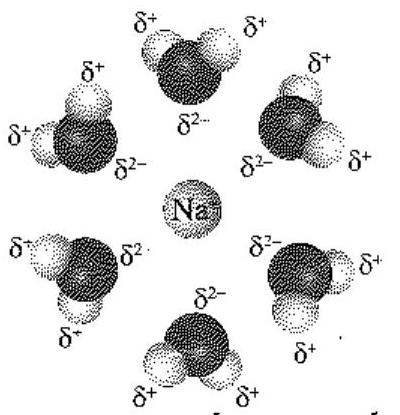
\includegraphics[max width=\textwidth, center]{2025_10_23_3f52bbaab6caa9e2ff75g-25}\\
21.16. Học sinh trả lời dựa vào các đặc điểm về liên kết trong phức chất và chất vô cơ đơn giản.
\end{itemize}

\section*{BÀl 22}
22.1. C. 22.2. A.\\
22.3. a) Học sinh viết 2 phương trình hoá học theo sơ đồ:

$$
\mathrm{M}^{3+} \rightarrow\left[\mathrm{M}\left(\mathrm{OH}_{2}\right)_{6}\right] \rightarrow\left[\mathrm{M}(\mathrm{OH})_{3}\left(\mathrm{OH}_{2}\right)_{3}\right]
$$

b) Phản ứng thứ hai (phản ứng thuỷ phân) tạo ra $\mathrm{H}_{3} \mathrm{O}^{+}$(hay $\mathrm{H}^{+}$).\\
c) Phản ứng thứ hai (phản ứng thuỷ phân) tạo ra $\left[\mathrm{M}(\mathrm{OH})_{3}\left(\mathrm{OH}_{2}\right)_{3}\right]$ là phức chất trung hoà nên ít tan trong nước. Phức chất này có dạng keo nên kết dính phù sa, cặn bã,... trong nước.\\
22.4. Màu xanh của dung dịch A là do sự hình thành phức chất $\left[\mathrm{Co}\left(\mathrm{OH}_{2}\right)_{6}\right]^{2+}(a q)$ theo phương trình hoá học:

$$
\mathrm{CoCl}_{2}(s)+6 \mathrm{H}_{2} \mathrm{O}(l) \rightarrow\left[\mathrm{Co}\left(\mathrm{OH}_{2}\right)_{6}\right]^{2+}(a q)+2 \mathrm{Cl}^{-}(a q) \quad\left(^{*}\right)
$$

Khi sấy khô băng giấy xảy ra phản ứng ngược với phản ứng (\textit{), tạo $\mathrm{CoCl}_{2}(s)$ màu hồng.\\
Khi băng giấy màu hồng tiếp xúc với mẫu vật có nước thì lại diễn ra quá trình (}).\\
22.5. (a) Đúng; (b) Sai; (c) Đúng (do có cấu trúc đối xứng, bền).\\
(d) Sai (Phức chất aqua $\left[\mathrm{M}\left(\mathrm{OH}_{2}\right)_{\mathrm{m}}\right]^{\mathrm{n}+}$ tan nên được ghi là $\left[\mathrm{M}\left(\mathrm{OH}_{2}\right)_{\mathrm{m}}\right]^{\mathrm{n}+}(a q)$ ).\\
22.6. (a), (b), (c), (e).\\
22.7. a) $\mathrm{CoCl}_{2}(s)+6 \mathrm{H}_{2} \mathrm{O}(b) \rightarrow\left[\mathrm{Co}\left(\mathrm{OH}_{2}\right)_{6}\right]^{2+}(a q)+2 \mathrm{Cl}^{-}(a q)$ màu xanh màu hồng\\
b) $\mathrm{CaCl}_{2}(s) \quad \xrightarrow{\mathrm{H}_{2} \mathrm{O}} \quad \mathrm{Ca}^{2+}(a q)+2 \mathrm{Cl}^{-}(a q)$ không màu không màu\\
22.8. Quá trình tạo dung dịch có màu xanh khi cho $\mathrm{CuO}(s)$ vào $\mathrm{H}_{2} \mathrm{SO}_{4}(a q)$ và có thể được mô tả như sau:\\
$\mathrm{CuO}(s)+\mathrm{H}_{2} \mathrm{SO}_{4}(a q)+5 \mathrm{H}_{2} \mathrm{O}(l) \rightarrow\left[\mathrm{Cu}\left(\mathrm{OH}_{2}\right)_{6}\right]^{2+}(a q)+\mathrm{SO}_{4}^{2-}(a q)$\\
22.9. (b), (c) có phản ứng thuỷ phân tạo $\mathrm{H}^{+}$(hay $\mathrm{H}_{3} \mathrm{O}^{+}$) như sau:

$$
\left[\mathrm{Al}\left(\mathrm{OH}_{2}\right)_{6}\right]^{3+}(a q)+\mathrm{H}_{2} \mathrm{O}(l) \rightleftharpoons\left[\mathrm{Al}(\mathrm{OH})\left(\mathrm{OH}_{2}\right)_{5}\right]^{2+}(a q)+\mathrm{H}_{3} \mathrm{O}^{+}(a q)
$$

hay $\left[\mathrm{Al}\left(\mathrm{OH}_{2}\right)_{6}\right]^{3+}(a q) \rightleftharpoons\left[\mathrm{Al}(\mathrm{OH})\left(\mathrm{OH}_{2}\right)_{5}\right]^{2+}(a q)+\mathrm{H}^{+}(a q)$.\\
22.10. (a) Sai; (b) Sai; (c) Đúng; (d) Đúng.\\
22.11. (a) Đúng; (b) Sai; (c) Sai; (d) Dúng.\\
22.12. a) Các quá trình diễn ra tương tự như sử dụng phèn nhôm - kali, tạo thành $\left[\mathrm{Fe}(\mathrm{OH})_{3}\left(\mathrm{OH}_{2}\right)_{3}\right]$ hay $\mathrm{Fe}(\mathrm{OH})_{3}$.\\
b) Có thể dùng dung dịch $\mathrm{Ba}(\mathrm{OH})_{2}$ và đún nóng nhẹ.\\
22.13. (a) Sai. Không tồn tại $\mathrm{Fe}^{3+}$ vì (I) là quá trình 1 chiều.\\
(b) Sai. Dựa vào giá trị hằng số cân bằng $\mathrm{K}_{\mathrm{C}}$ để lập luận.\\
(c) Đúng. Do khi đó trong dung dịch có thêm phản ứng (II).\\
(d) Đúng.\\
22.14. (a) Đúng; (b) Sai; (c) Đúng;\\
(d) Sai (phức chất ở dạng ion là phức chất tan trong nước).

22,15. C. Các phát biểu đúng gồm (2), (3), (4) và (6).


\end{document}